\documentclass[11pt, oneside]{article}   	% use "amsart" instead of "article" for AMSLaTeX format
\usepackage{geometry}                		% See geometry.pdf to learn the layout options. There are lots.
\geometry{letterpaper}                   		% ... or a4paper or a5paper or ... 
%\geometry{landscape}                		% Activate for rotated page geometry
%\usepackage[parfill]{parskip}    		% Activate to begin paragraphs with an empty line rather than an indent
\usepackage{graphicx}				% Use pdf, png, jpg, or eps§ with pdflatex; use eps in DVI mode
								% TeX will automatically convert eps --> pdf in pdflatex
\graphicspath{ {./images/} }
\usepackage{amssymb}

%SetFonts

%SetFonts
\usepackage{subcaption} %  			direttiva

\title{Sicurezza informatica}
\author{Federico Zhou}
%\date{}							% Activate to display a given date or no date

\usepackage{float}

\begin{document}
\maketitle
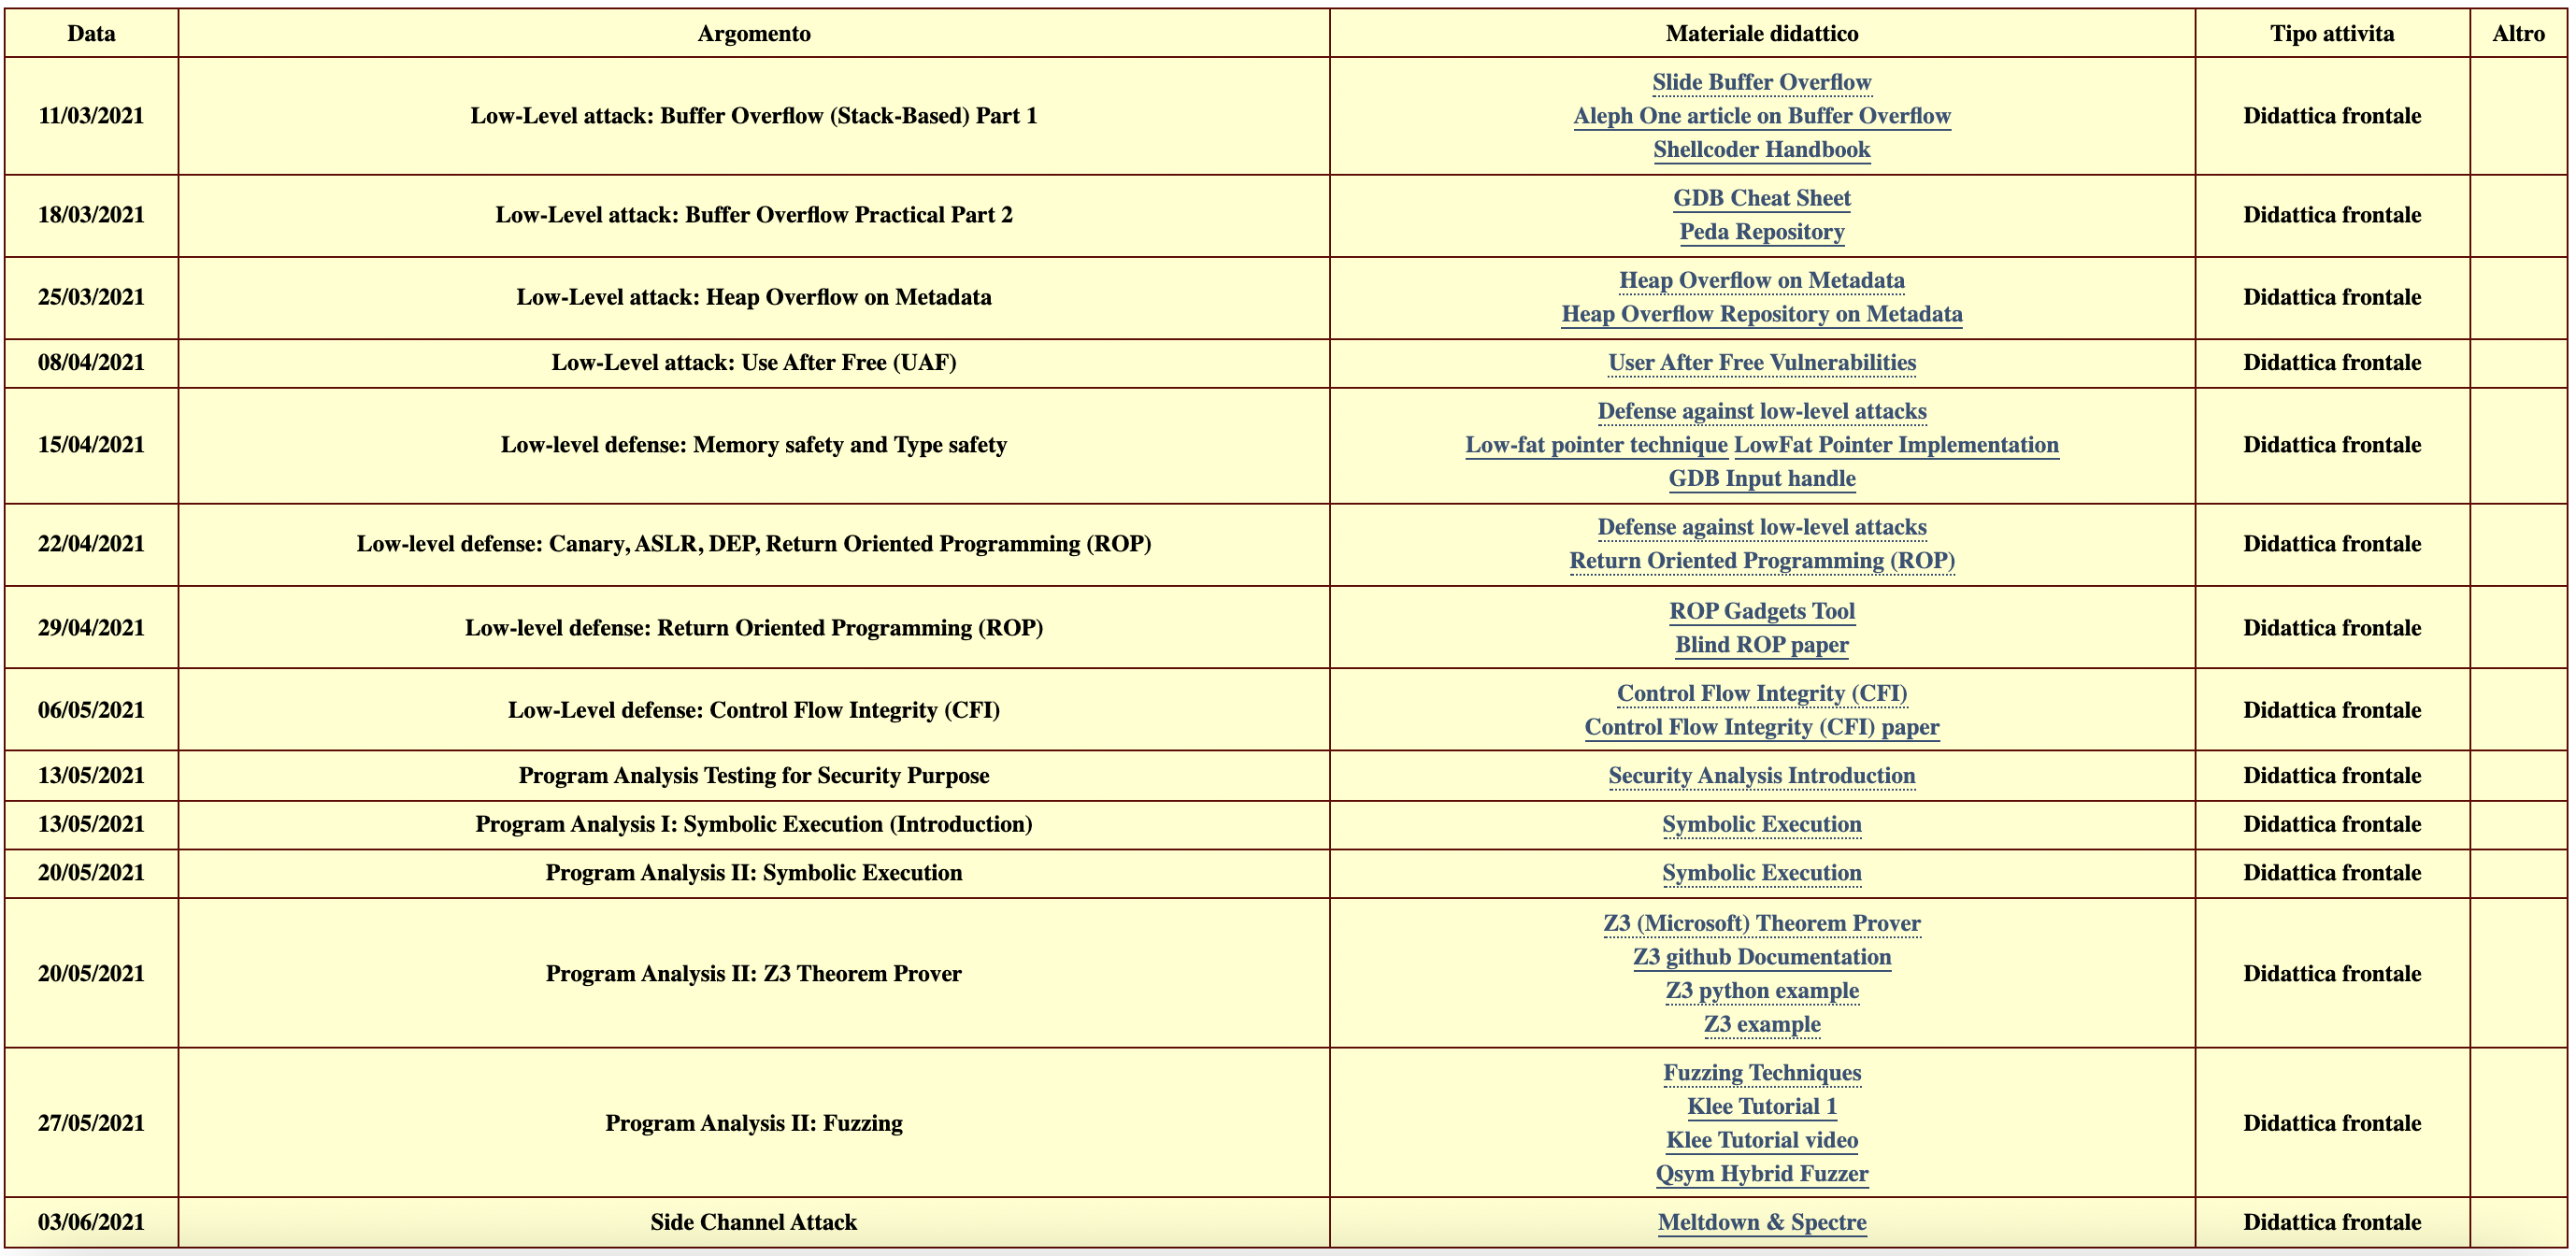
\includegraphics[scale=0.3]{programma}
%\
\section{Buffer overflow}
A buffer overflow is a bug that affects low-level code, normally a program would crash but an attacker can alter the situation \emph{to steal informations, corrupt valuable information or run an attacker's code of choice.}\\
They are relevant because C and C++ are still popular, and buffer overflow attacks stil happen regularly.
They have a long history and there are many approaches to defend against them.\\
The levels in which we can act to defend against them, the compiler, the OS, or the architecture.
\subsection*{Memory Layout (32bit, Linux)}
In pile in a 32 bit system, Linux or Intel 32-bit the addresses range from 0x00000000 to 0xBFFFFFFF.\\
The stack, which grows downwards, is the place in which activation records are stored, together with the heap they are created in runtime. The heap is managed with malloc, calloc, free and grows upwards, and contains variables. The text segment contains the instructions.
\begin{center}
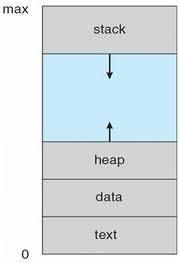
\includegraphics[scale = 0.5]{heapstack}
\end{center}
Memory operations make the memory grow upwards, this makes overwriting the SFP possible, allowing memory errors.
\begin{center}
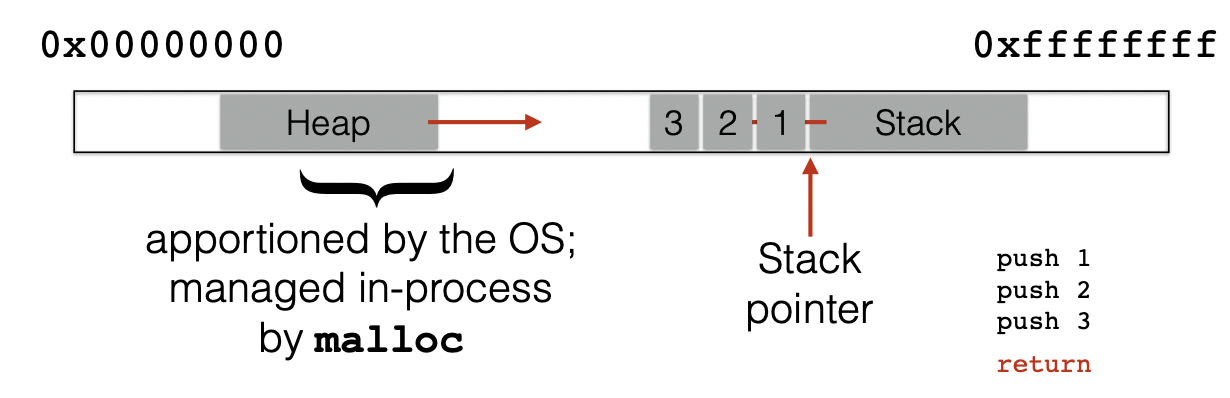
\includegraphics[scale = 0.5]{memory5}
\end{center}
\begin{center}
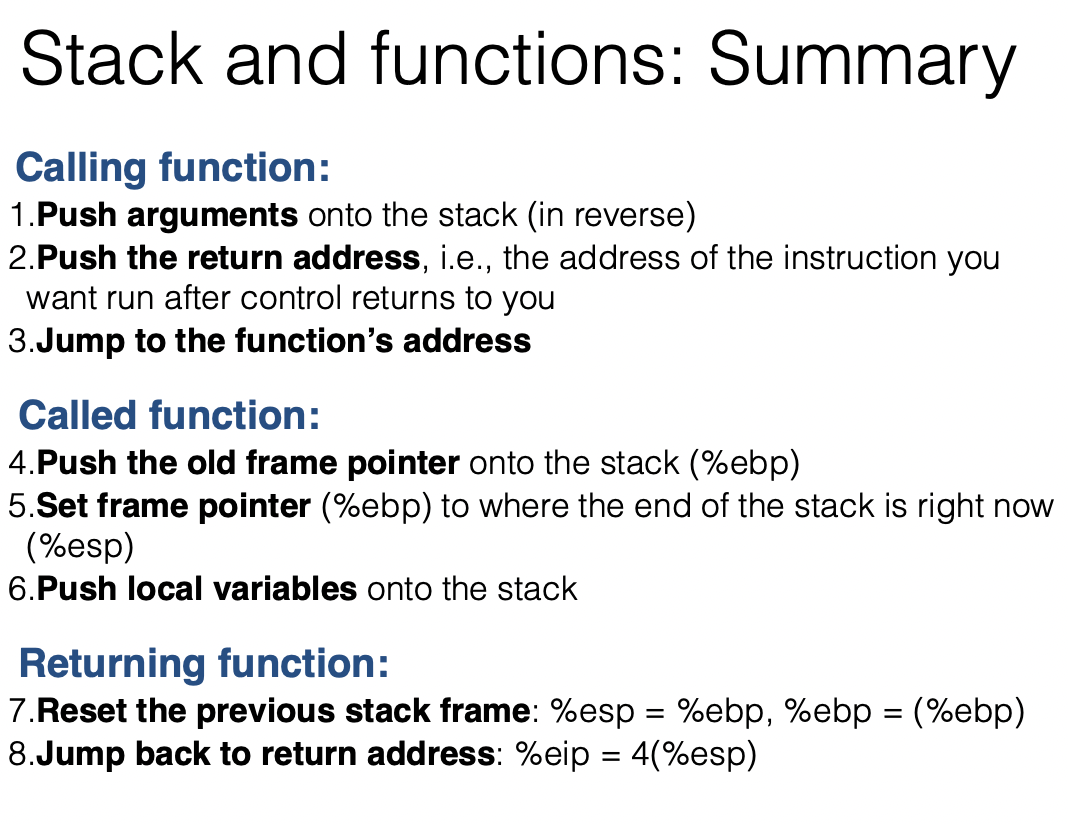
\includegraphics[scale = 0.4]{memory6}
\end{center}
Firstly let's talk about buffers, buffers are a contiguous piece of memory associated with a variable or a field, these are common in C. By overflowing a buffer we can put more into the buffer than it can hold.\\
In this example: BUF1 (which is big [24], is copied into BUF[20], since memory operation increases the heap upwards, it is possible to overwrite the SFP, causing a segmentation fault error.
\begin{center}
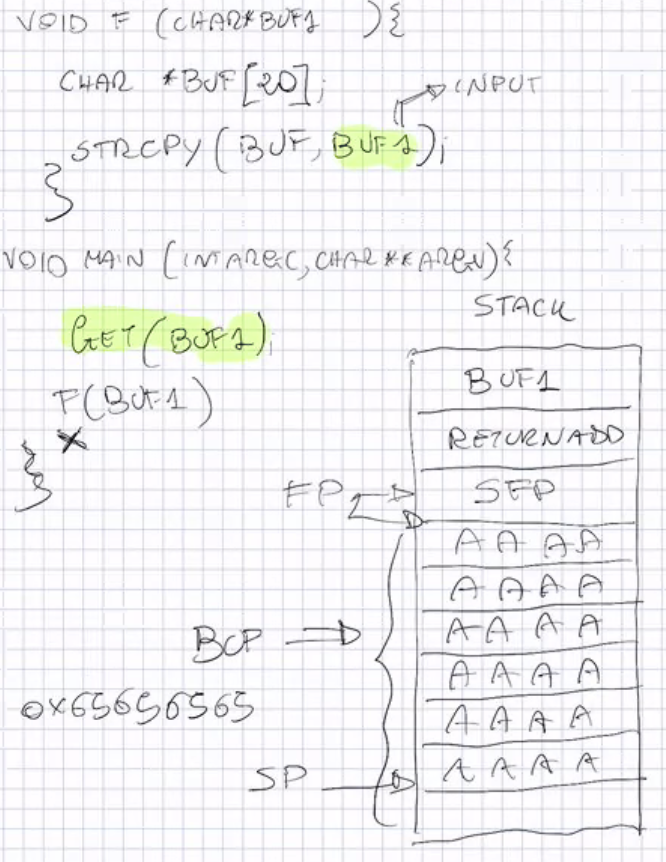
\includegraphics[scale = 0.5]{memory2}
\end{center}
\emph{We have crashed the system, but how can we exploit this?}\\
Note that strcpy will let you write as much as you want till a terminator character, we could introduce particularly crafted code to wreak havoc.\\
If instead of AAAA (which is: 0x65656565) we introduce code which alters the normal execution of the program, overwriting the return address.\\
How do we build the injection vector?
\begin{center}
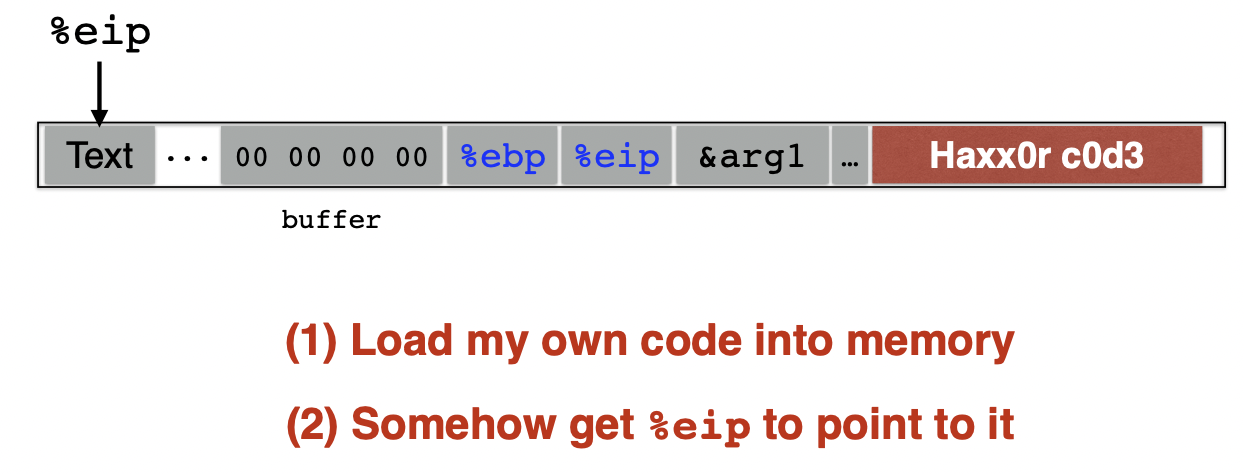
\includegraphics[scale = 0.4]{injcode}
\end{center}
{\footnotesize Note that the "disallocation" only consists in a subtraction of the reference pointer, the data remains\\
We introduce arbitrary shellcode, and by hijacking the return address we can execute code we want}\\
We can only load machine code into memory, which are instructions already compiled and ready to run, since we're trying to give the attacker general access to the system, the best candidate is the general-purpose shell. \\The shellcode is carefully crafted in the format \emph{[SHELLCODE][ADDRESSBUF] = Attack Vector} and it is copied with the function call "strcpy".
It is fundamental we get to know the [ADDRESSBUF], since if we don't an unrecognised instruction is going to run and C is gonna throw an IllegaArgumentException.\\
{\footnotesize Shellcode: machine code-that we want to execute-to run a shell}\\
The idea: we can't insert a "jump to my code" instruction, so we hijack the saved \%eip. Since we don't know the desired \%eip address we'll have to:\begin{itemize}
\item Try a lot of different values, upwards of $2^{32}$ possible answers\\
\item Without address randomisation, the stack always start from a fixed address, and it doesn't grow very deeply.
\end{itemize}
How do we increase the chances to execute our shell-codes ?\\
Introduce the NOPSLED: 0x90 is a NOP instruction, single byte instruction which does nothing.
We can fill our vector buffer of NOP operations, thus increasing the chances of execution
\begin{figure}
\begin{subfigure}{0.4\linewidth}
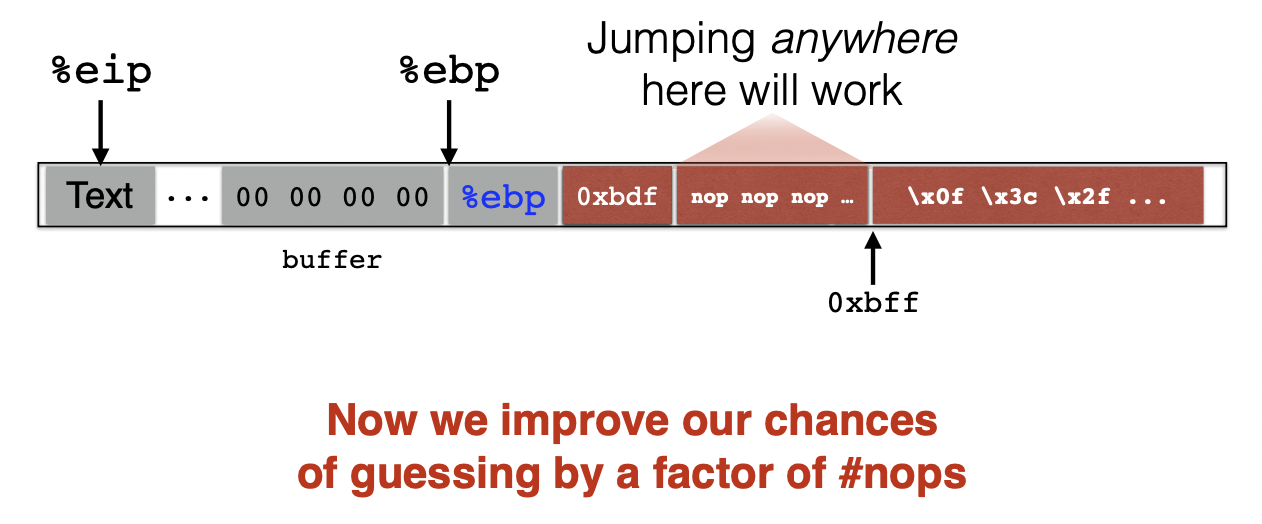
\includegraphics[width=\linewidth]{nop}
\end{subfigure}
\hfill
\begin{subfigure}{0.4\linewidth}
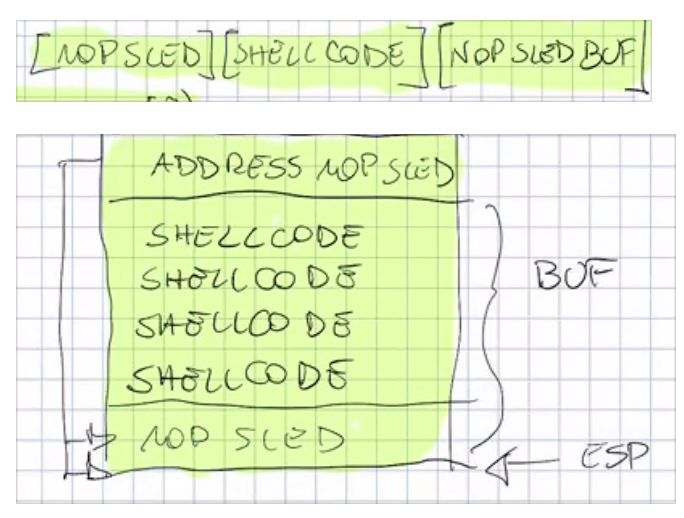
\includegraphics[width=\linewidth]{nopsled}
\end{subfigure}
\end{figure}
Depending on the size of the buffer, we have to size our shellcode. The size depends on the allocated space by the target char array in strcpy.\\ \emph{char BUF[20]; strcpy(BUF, BUF1); size of the buffer to work with is 20}\\
The computer by itself has protections, mainly towards the \textbf{returnAddress}, such as canary, nx

\section*{Heap vs Stack}
Let's take an overlook over the differences between the Stack and the Heap:
\begin{itemize}
\item The stack:\\
- has a fixed memory allocation, which is only known at compile time\\
- inside it reside local variables, return addresses, functions args\\
- it's very fast and automatic, and it is managed by the compiler
\item The Heap:\\
- has dynamic memory allocation, known at runtime\\
- inside it reside objects, big buffers, structs, persistence and larger objects\\
- it's slower, manual, managed by the programme
\end{itemize}
The Heap is a pool of memory used to dynamic allocations, managed with:\\
- \emph{malloc()}: to allocate memory on the heap\\
- \emph{free()}: to release memory on the heap\\\begin{center}
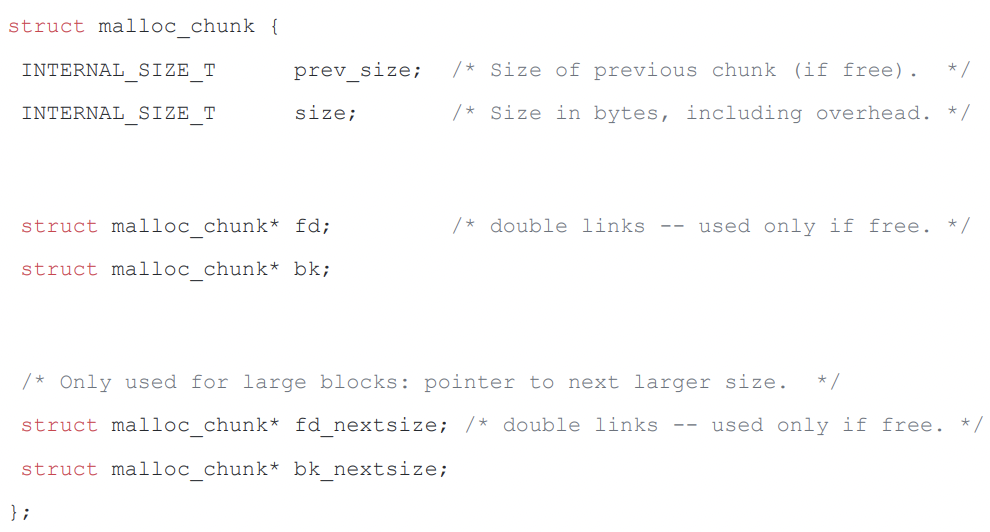
\includegraphics[scale = 0.6]{heap}
\end{center}
Let's see an overview of a heap chunk:
\begin{center}
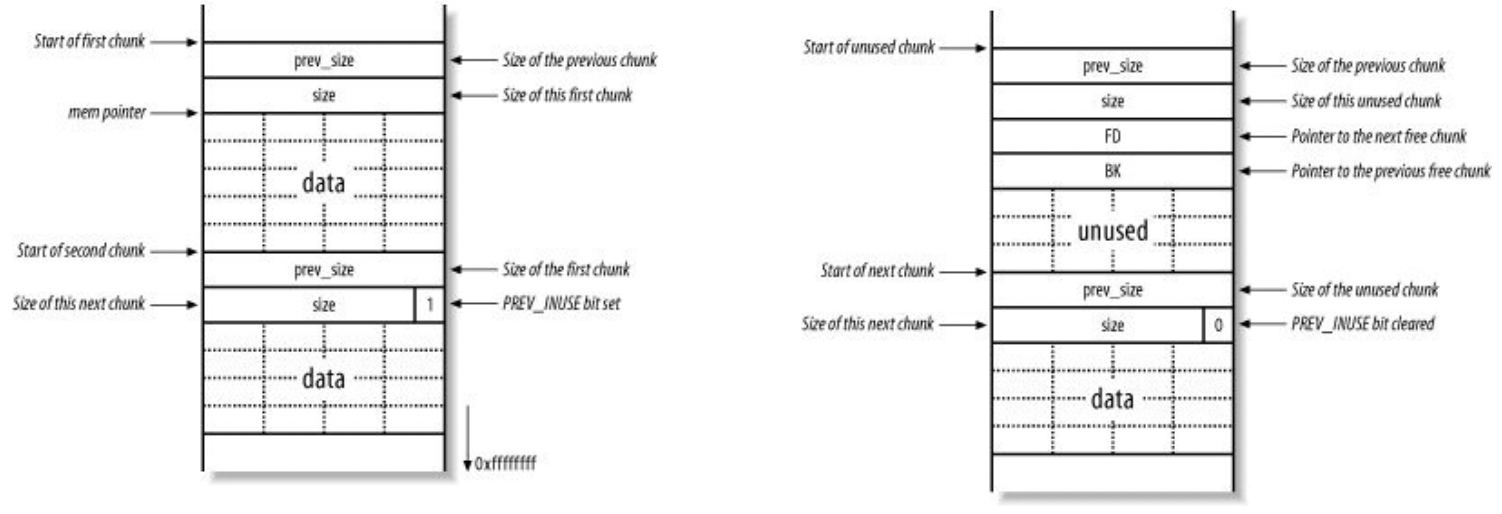
\includegraphics[scale = 0.6]{heap2}
\end{center}
The chunk is a part of the memory allocated in the heap. Alongside the data, it also contains metadata:
\begin{itemize}
\item prev\textunderscore size: contains the size of the pervious chunk 
\item size: it is also equipped with a bit-switch \emph{PREV\textunderscore INUSE}.
It contains the size of the previous chunk.
\item FD: the pointer to next free chunk
\item BK: the pointer previous free chunk
\end{itemize}

The heap grows upwards.
\emph{prev\textunderscore size and size} concurrently form the metadata section of the heap chunk.
When we call \emph{P = malloc(128)}, the pointer points to memPointer, just below the metadatas.\\\\
\emph{The free function}
When \emph{free(p)} is used, the LSB of the size field in the metadata of the next chunk is cleared. Additionally the prev\textunderscore size field of the next size will be set to the size of the chunk we are currently freeing. \\
The system keeps multiple lists of the freed chunks, which can be of different size, when a chunk is freed, we can verified if the previous chunk is freed to, and if it is we can unify them into a single bigger chunk.\\
When an allocation request is made, the system looks into the first free chunk that has a size \(\geq\) than the size requested. If no free chunk is found, the top chunk will be used.\\\\
AV\textunderscore TOP è il riferimento al top chunk; rappresenta lo spazio rimanente. Quando solleviamo una memory request e lo spazio nello heap è esaurito \emph{eg. malloc(256)} il topchunk è diviso in due, e rispettivamente le parti diventano topchunk e la parte richiesta.\\
When we deallocate a chunk, we use an unlink function, this leaves an opening for us, the attacker. By hijacking the two metadata values it allows us to write an arbitrary value to an arbitrary location.
\begin{center}
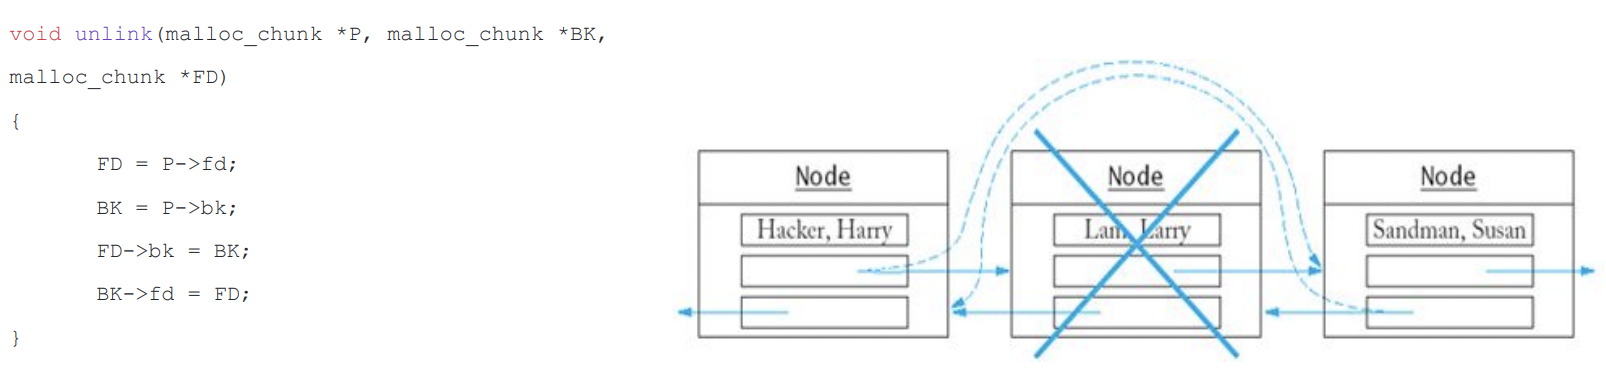
\includegraphics[scale = 0.6]{atk1}
\emph{the intended process}\\
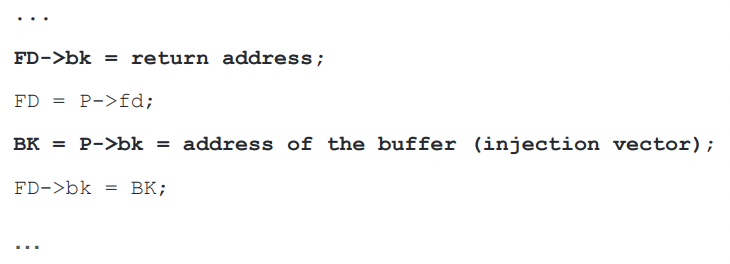
\includegraphics[scale = 0.6]{atk2}\\
\emph{malicious code which allows us to manipulate the BK}
\end{center}
Unfortunately this technique no longer works, the current unlink function verifies beforehand the values
We can however look for other flaws:

\subsection*{House of Force vulnerability}
Conditions:
\begin{itemize}
\item It requires 3 malloc, more precisely a malloc that allows us to overwrite the top chunk, one malloc with a user controllable size and another call to malloc.
\item 1 (or 2) strcpy
\end{itemize}
\subsection*{Use after free vulnerability}
Use after free vulnerability are vulnerabilities that happen when a pointer to an object that has been freed is deferenced. This can lead to information leakage, and furthermore the attacker could also modify unintended memory locations that can potentially lead to code execution.\\
A prime candidate for an attack is a dangling pointer. Dangling pointer happen when a pointer, which was previously the target of another pointer is deleted, leaving the other pointer dangling.\\
\begin{center}
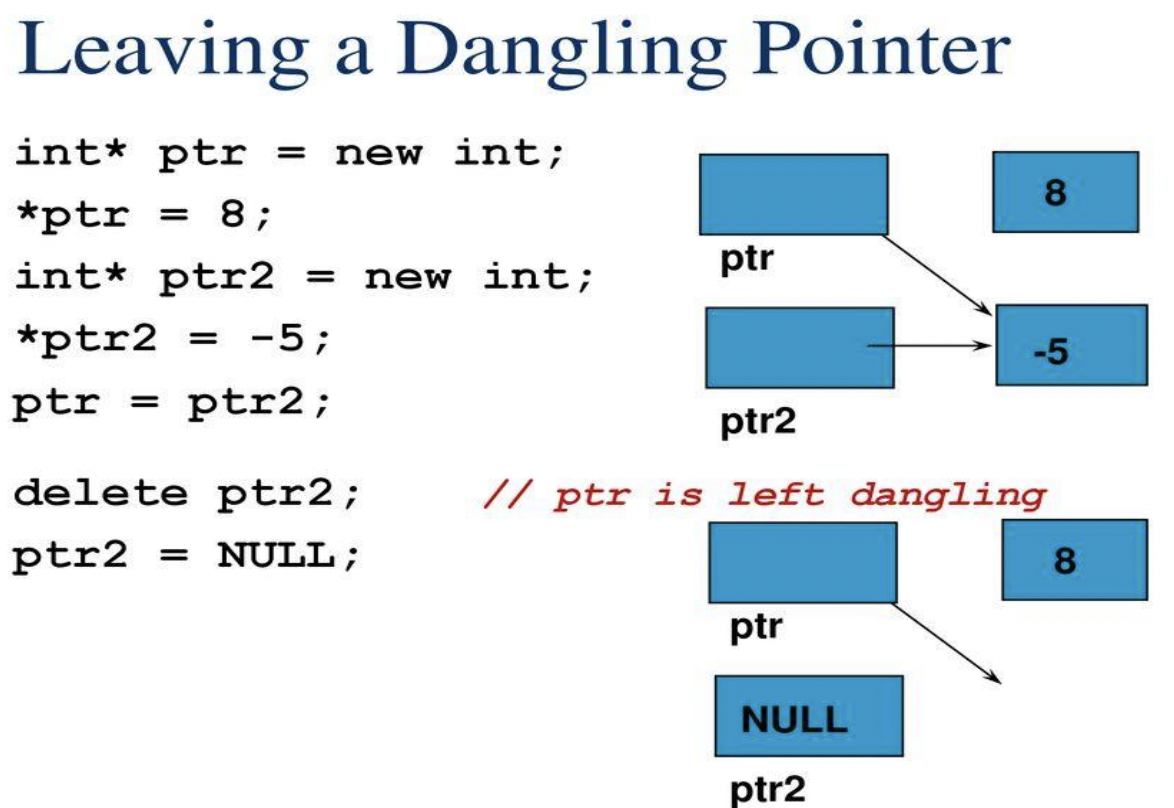
\includegraphics[scale = 0.6]{dpointer}
\end{center}
This happens because in C the entire management of pointers is left to programmers. In java this issue doesn't manifest itself because unused/unallocated memory spaces are collected by the garbage collector.\\\\
Let's see an actual example of user after free vulnerability
\begin{center}
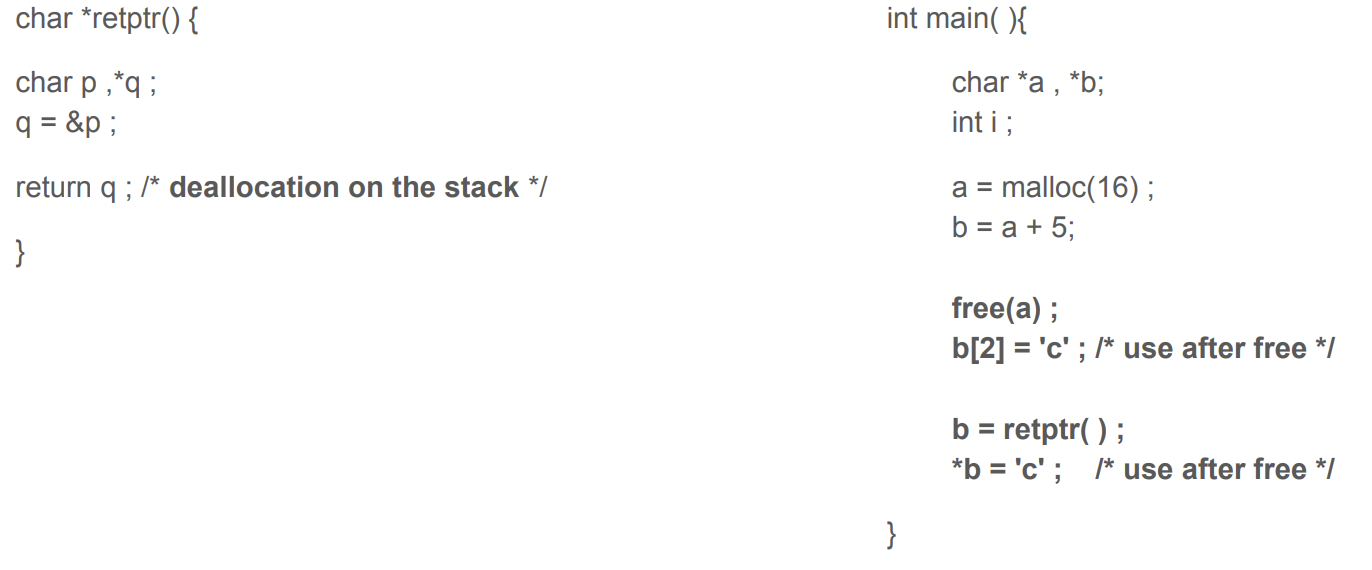
\includegraphics[scale = 0.6]{usafter}
\end{center}
In this example, a is a contiguous memory space long 16 bytes, b points to a location inside of a.\\
b, after using \emph{b[2] = 'c'} is able to modify a memory portion of a after it has been freed (de-allocation).
\begin{center}
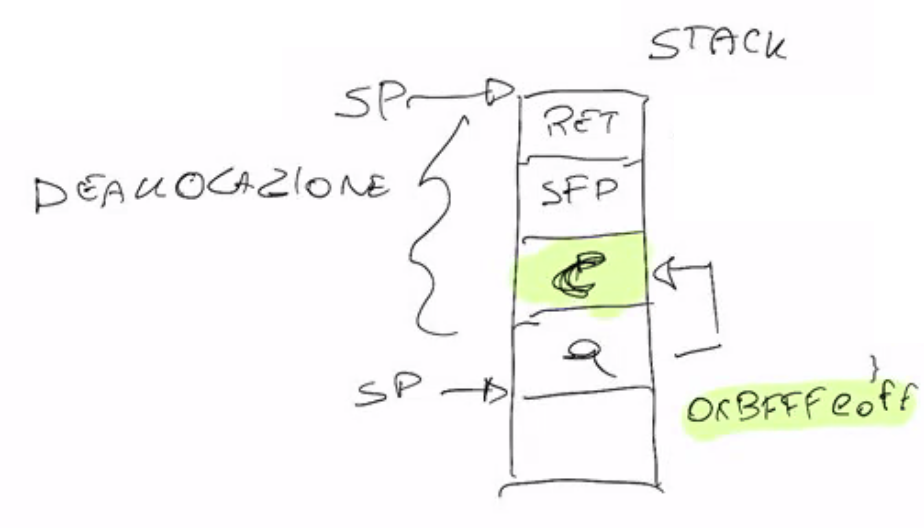
\includegraphics[scale = 0.6]{usafter2}
\end{center}
b punta a una porzione dello stack che è stata deallocata. chiamando *b = 'c' modifichiamo una porzione dello stack che è stata deallocata precedentemente (nello stack p diventa c).

\section*{Defence and mitigation mechanisms}
All these attacks have in common a couple of characteristics:\begin{itemize}
\item The attacker is able to control some data that is used by the program
\item The use of data permits unintentional access to some memory area in the program past a buffer, or to an arbitrary position on the stack.
\end{itemize}
So what can we do to \emph{mitigate} these vulnerabilities?\\
First of all it's important we mention that we are not going to implement solutions which are going to leave us with a type safety and memory safety language. We are only going to implement mechanisms which are going to make the exploitation of these vulnerabilities too costly/time consuming.\\\\
Type safety and memory safety are two fundamental mechanisms which can help us mitigate these vulnerabilities, these properties, if met, ensure an application is immune to memory attacks. Languages such as C and C++ don't implement memory and type safety due to its efficiency load, other languages that do are JAVA or Python.\\\\
\emph{So what can we actually do?}
\begin{itemize}

\item Automatic defences:\\
these defences are specific to the compiler and help protect the return address and
- Stack canaries: protects the return address from hijacking.\\
More precisely a stack canary is a value placed on the stack such that a stack-buffer overflow will overwrite it before corrupting the return address. The buffer overflow can then be detected by verifying the integrity of the canary before performing the return. It is fundamental that the stack canary remains confidential, otherwise the attacker could just copy it and hijack the control flow anyway
\begin{center}
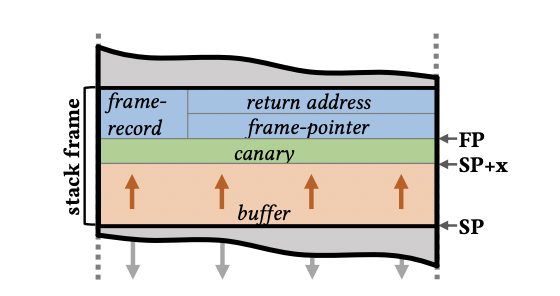
\includegraphics[scale = 0.6]{canary}
\end{center}
- Address space layout randomisation \textbf{(ASLR)}: is a memory-protection process for operating systems that guards against buffer-overflow attacks by randomising the location where system executables are loaded into memory. \\Being able to determine beforehand the position of processes and functions in memory makes exploitation easier, and ASLR is able to put address space targets in unpredictable locations, the attacker won't be able to identify the correct address space, making the application crash and notifying the system.
\item Return-oriented programming \textbf{(ROP)}attacks are based on the technique that allows the attacker to hijack the program control flow by executing machine code instructions present in the machine's memory. \\
This is done by manipulating the call stack by exploiting vulnerabilities in a program, typically a buffer overflow.\\
Control Flow Integrity \textbf{(CFI)} are mechanisms implemented to prevent a variety of attacks based on the redirection of the control flow of the program.
\item Secure coding are a set of practises that applies to security considerations that help defend against vulnerabilities, bugs and exploits. Secure coding introduces safeguards which reduce or eliminate the risk of leaving security vulnerabilities in the code, most important of which are \textbf{memory safety and type safety}
\end{itemize}

\section*{Memory Safety}
Memory safety is a fundamental principle which helps mitigate C's vulnerabilities, in particular to guarantee a degree of memory safety in C we can impose to:
\begin{itemize}
\item only create pointer through standard means
\begin{center}
p  = malloc(...), or p = \&x, or p = \&buf[5] etc.
\end{center}
item only use pointers to access memory that "belong", that is within the bound of that pointer and of the type that corresponds. (int* to integers, char* to characters).
\end{itemize}
This essentially combines two principles: \emph{temporal safety and spatial safety}.


\subsection*{Spatial Safety (in the heap)}
Pointers are viewed as triples $(p, b, e)$ where:
\begin{itemize}
\item $p$ is the actual pointer
\item $b$ is the base of the memory region it may access
\item $e$is the extent (or the bounds) of the region
\end{itemize}
The deferenced access shall be allowed iff $ b \leq p \leq e - sizeof(typeof(p))$. \\ An implementation of a spatial safety compliant memcpy:
\begin{center}
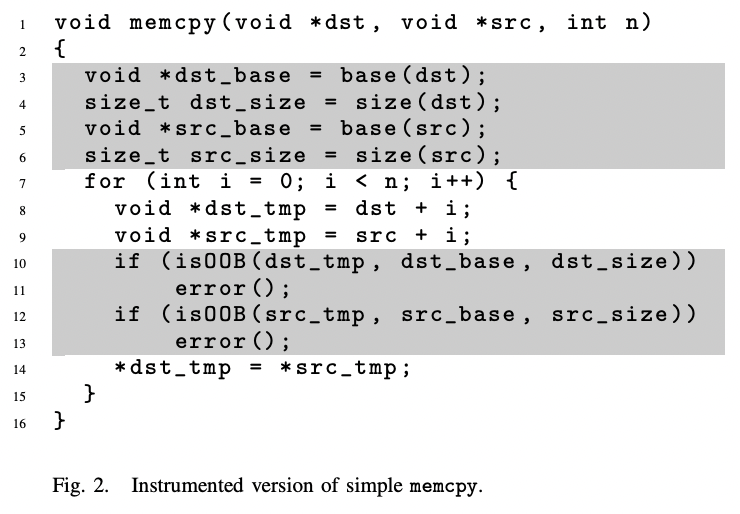
\includegraphics[scale = 0.6]{memsef}
\end{center}


\subsection*{Temporal safety}
Memory regions can either be defined or undefined:\begin{itemize}
\item defined means allocated (and active)
\item undefined means allocated, uninitialised, or deallocated\\
A temporal safety violation occurs when an attacker tries to access undefined memory space
\item spatial safety assures that an accessed region is legal
\item temporal safety assures that region is still in play
\end{itemize}
When a free function is called, the pointer towards that region is freed up, but the data remains in the stack, just unreferenced. The garbage collection's job is the memory management, its main function is to reclaim memory which was allocated by the program, but is no longer referenced.\\
The aim is to implement mechanisms similar to the garbage collector, but not quite; we want to protect vulnerable portions of the memory. The garbage collectors are demanding in terms of resources.\\\\
But why would we want to use a language that is \textbf{not memory safe and type safe}?\\
The easiest way to avoid all these vulnerabilities would be to use a \textbf{memory safe language}, languages that are \textbf{type safe are even better.} 
\begin{center}
\textbf{Type safety  $>$ Memory Safety}
\end{center}
\subsection*{Type safety in C}
The main reason is that C and C++ are \textbf{here to stay}, while not memory safe, writing memory safe programs is possible.\\The problem of type safety and memory safety has been known for more than 20 years, the limiting factor has always been \textbf{performance}  (around 12x and 17x overhead). Furthermore adding type safety would also make C and C++ much slower. \\
Type safety enforcement is expensive, the most important mechanisms are 
\begin{itemize}
\item \textbf{Garbage collection} which avoids temporal violations, but uses much more memory
\item \textbf{Bound} and null pointer checks which avoids spatial violations
\item \textbf{Hiding representation} may \textbf{inhibit optimisation}\\
technique such as C-style casts, pointer arithmetic, \& operators would not be allowed
\end{itemize}
\subsection*{So what can we do in C?}
\begin{itemize}
\item Compiler could add code to \textbf{check for violations}\\
An out-of-bounds access would result in immediate failure just like an \emph{ArrayBoundsException} in Java.
\item \textbf{No dangling pointers}\\
Accessing a freed pointer violates temporal safety, accessing uninitialised pointers is also not OK:
\begin{figure}[H]
\begin{subfigure}[H]{0.5\linewidth}
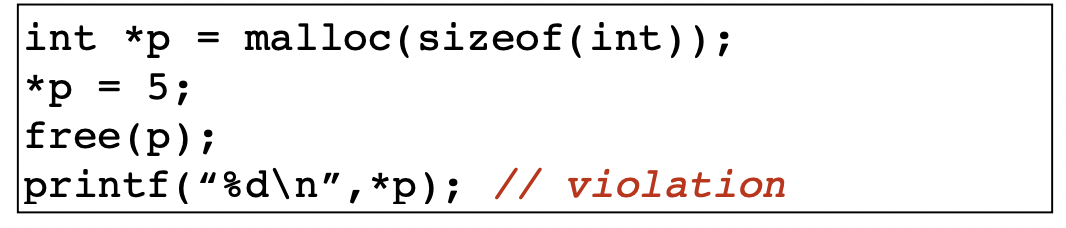
\includegraphics[width=\linewidth]{sef1}
\end{subfigure}
\begin{subfigure}[H]{0.5\linewidth}
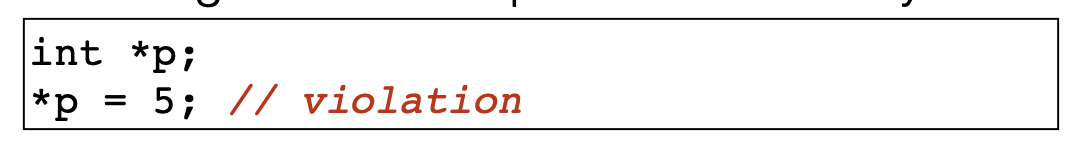
\includegraphics[width=\linewidth]{sef2}
\end{subfigure}%
\end{figure}
\item \textbf{Type safety}\\
Each objects shall be ascribed a type (int, pointer to int, pointer to function).\\
Operations on he objects shall be always compatible with the object's type. Type safe programs can't encounter runtime errors. Type safety implies that objects shall always have a compatible types, while guarantee bounds compliance
\begin{center}
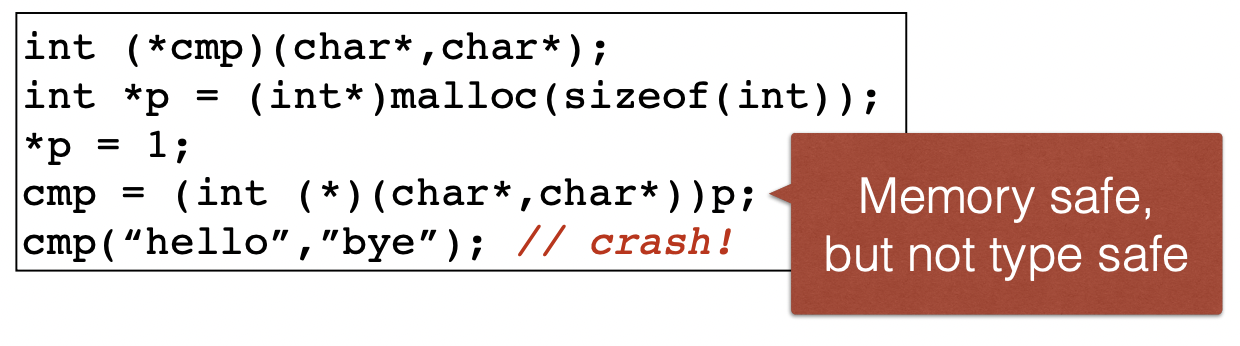
\includegraphics[scale = 0.6]{tsef}
\end{center}
\end{itemize}

\subsection*{So how can we guarantee a degree of type safety in C?}
Using \textbf{enforce invariants}, are properties which cannot be violated by type, by enforcing invariants in the program. Most notably is the enforcement of \textbf{abstract types}, which characterised modules. It keep the \textbf{representation of the modules hidden from others}. This guarantee a \textbf{degree of isolation} from the rest of the system.\\\\
Type-enforced invariants can relate to security properties, by expressing stronger invariants about data's privacy and integrity we can mitigate type mismatch exploits, such as the following in Java.
\begin{center}
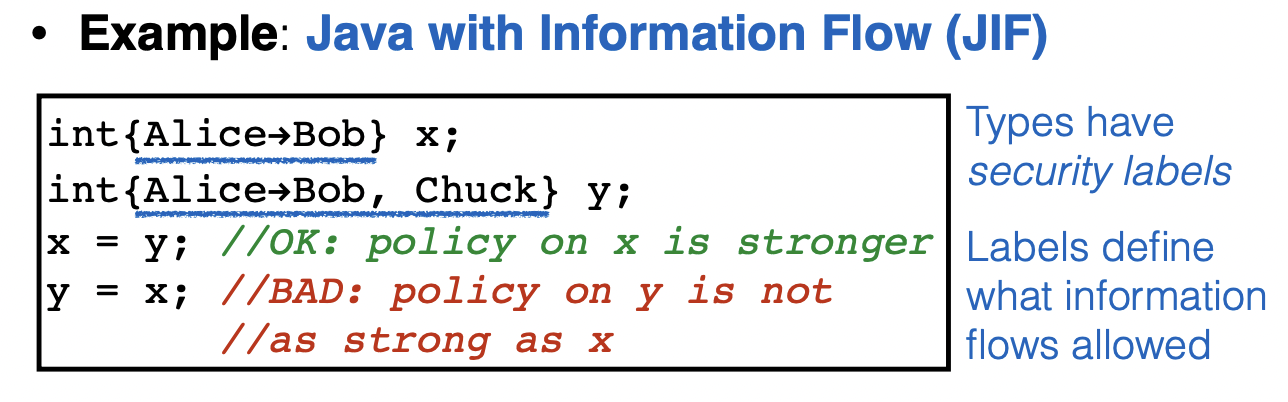
\includegraphics[scale = 0.6]{alice}
\end{center}
All of these mechanisms concurrently compose the security by design principle, which means that the language and its capabilities are foundationally secure. In this approach security is built into the system, not mitigating since the design stage notable vulnerabilities.\\
There are already languages which provide similar features to C, while remaining type safe, notable examples are Google's Go, Mozilla's Rust, Apple's Swift.

\subsection*{Other defensive strategies:}
These are complementary, they mitigate bugs but can't shut them out entirely
\begin{itemize}
\item Make the bug harder to exploit: introduce more steps, to make them difficult or impossible
\item Avoid the bug entirely: practice secure coding practices, advanced code review and testing
\end{itemize}
To implement these, let's recall the steps of a stack smashing attack:
\begin{itemize}
\item Putting the attacker code into the memory. The shellcode must also not contain zero (it is interpreted by the machine as a string terminator)
\item Getting \emph{\%eip} to point at the shellcode
\item Finding the return address (by guessing the raw address)
\end{itemize}
To make these attacks steps more difficult we can use libraries, compiler mechanisms and the operating system. We are trying to fix the architectural design, and not the code.

\section*{Overflows detection}
\subsection*{Stack canaries}
Managed by the compiler, canaries work by protecting the return address by detecting any change that could have harmed the stack's integrity. The canaries are placed inside the stack in a protected memory section between user and system variables. \\The canary's value has to be random, and unaccessible by the attacker otherwise it could be overwritten with the same value.
The canary is introduced when the function is called, using a machine code function called \emph{push canary}
\begin{center}
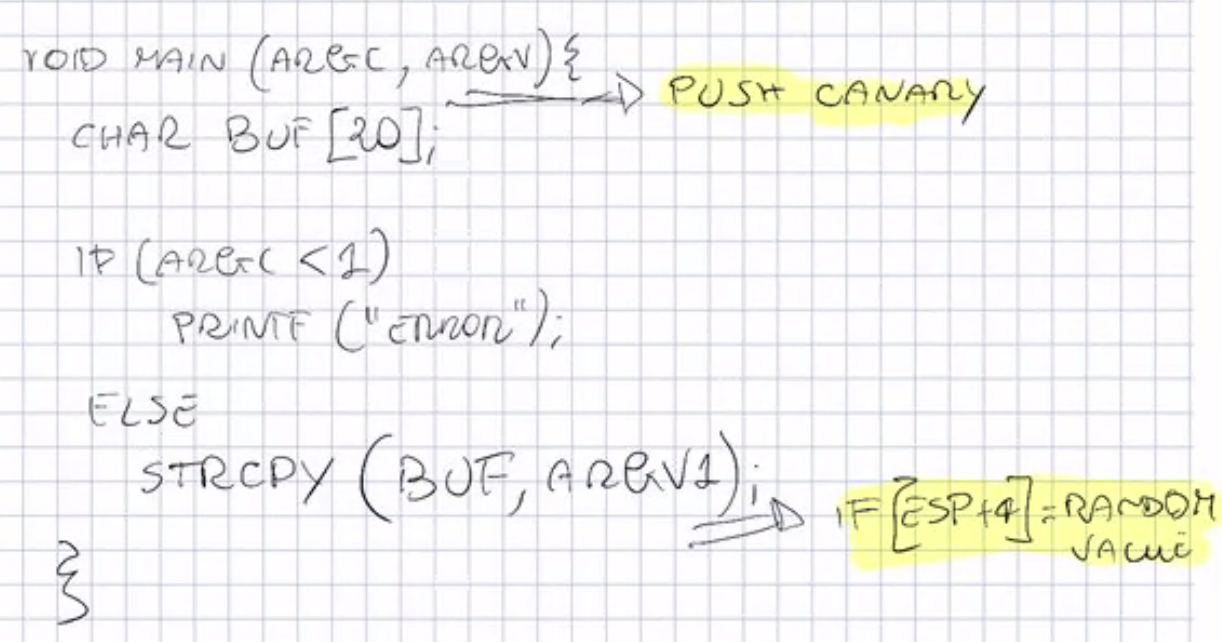
\includegraphics[scale = 0.6]{pushcanary}
\end{center}
Before calling the \emph{ret} the value of the canary is checked, raising errors if it's not correct.
The values the canary can assume are these:
\begin{center}
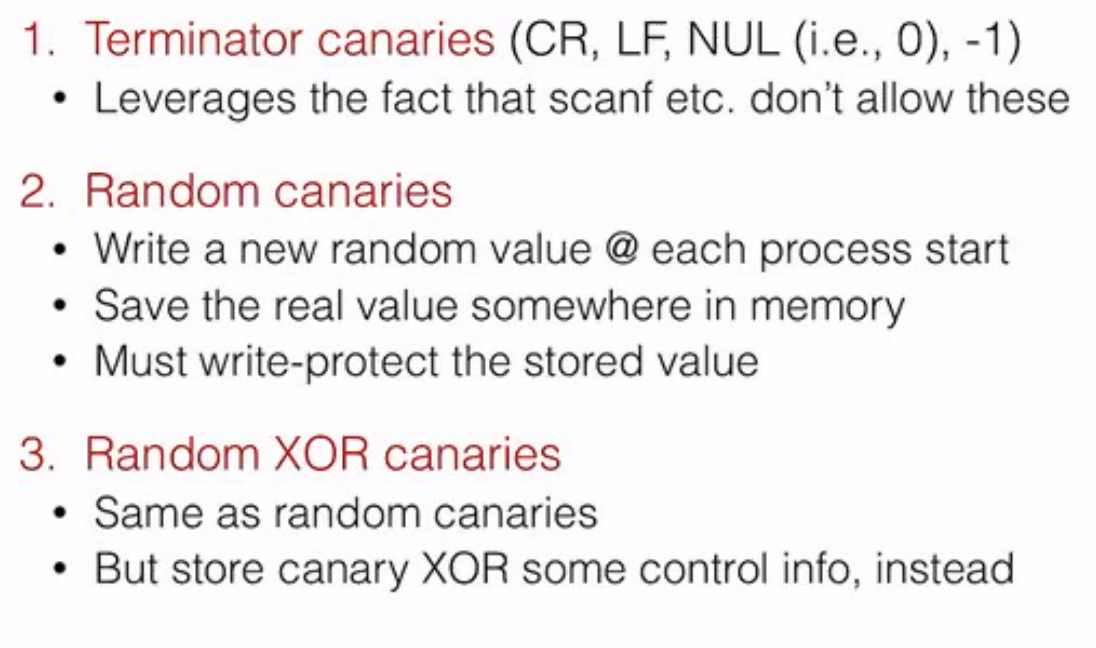
\includegraphics[scale = 0.6]{values}
\end{center}
3. Random XOR canaries work by doing:
\begin{enumerate}
\item $[ret$ $XOR$ $canaryValue]$ to produce che canary value
\item $[ret$ $XOR$ $canaryValue]$ the verify the canary value
\end{enumerate}
This works due to the nature of XOR, calling it two times gives us the initial value

\subsection*{DEP | Data Execution Prevention}
This defence works by making the stack and heap memory space non-executable. Attackers bypassed this defence by having the shellcode point to system libraries in an attack called \emph{return-to-libc}.\\ lib-c libraries are used by the gcc compiler, meaning they are always available.\\\\
To use this attack, system is called. System is a function that has argument a terminal command. In order to work with this vulnerability, we need to first: call the system function, and two: have it run a meaningful command. This is done by placing the command next to the system call. The injection vector is modified in the following way.
\begin{center}
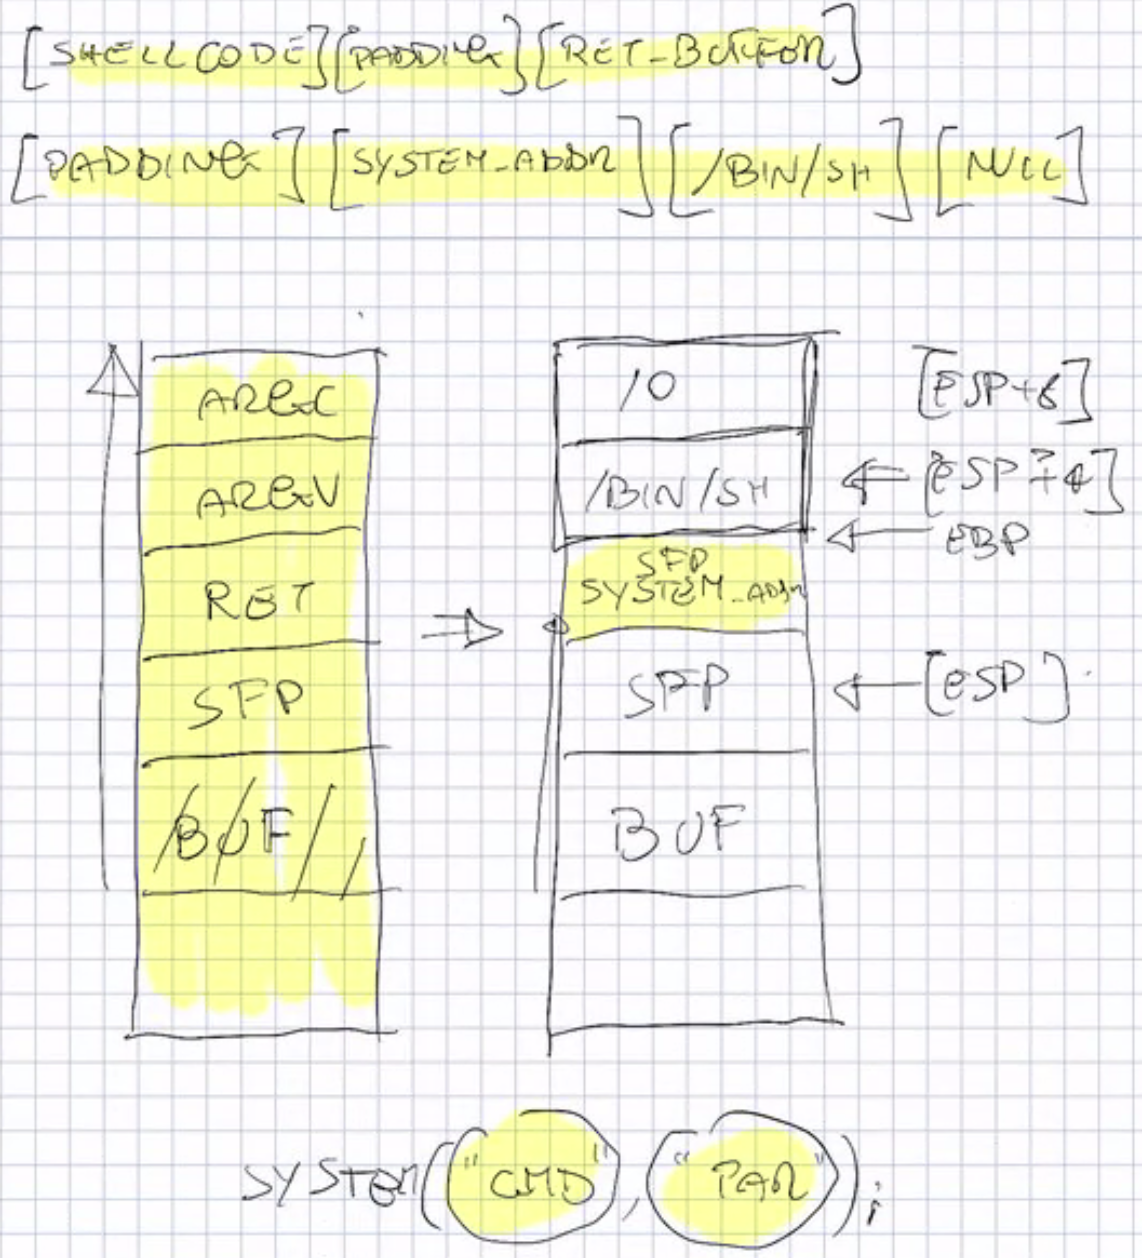
\includegraphics[scale = 0.5]{libc}
\end{center}
Defence strategies mitigated the \emph{return-to-libc attack} by introducing \emph{Address-space Layout Randomization or ASLR} which places standard libraries and other elements in memory in random places, making them harder to guess. It also has some caveats:
\begin{itemize}
\item Only shifts the offset of memory areas, not particular locations within those areas
\item May not apply to program code, but only libraries
\item Need sufficient randomness, otherwise it could be brute forced.\\
this makes this technique more promising on 64-bit systems
\end{itemize}
When we talk about \emph{cat and mouse} we mean the game of cat and mouse being played by attackers and the defence specialists.
\begin{center}
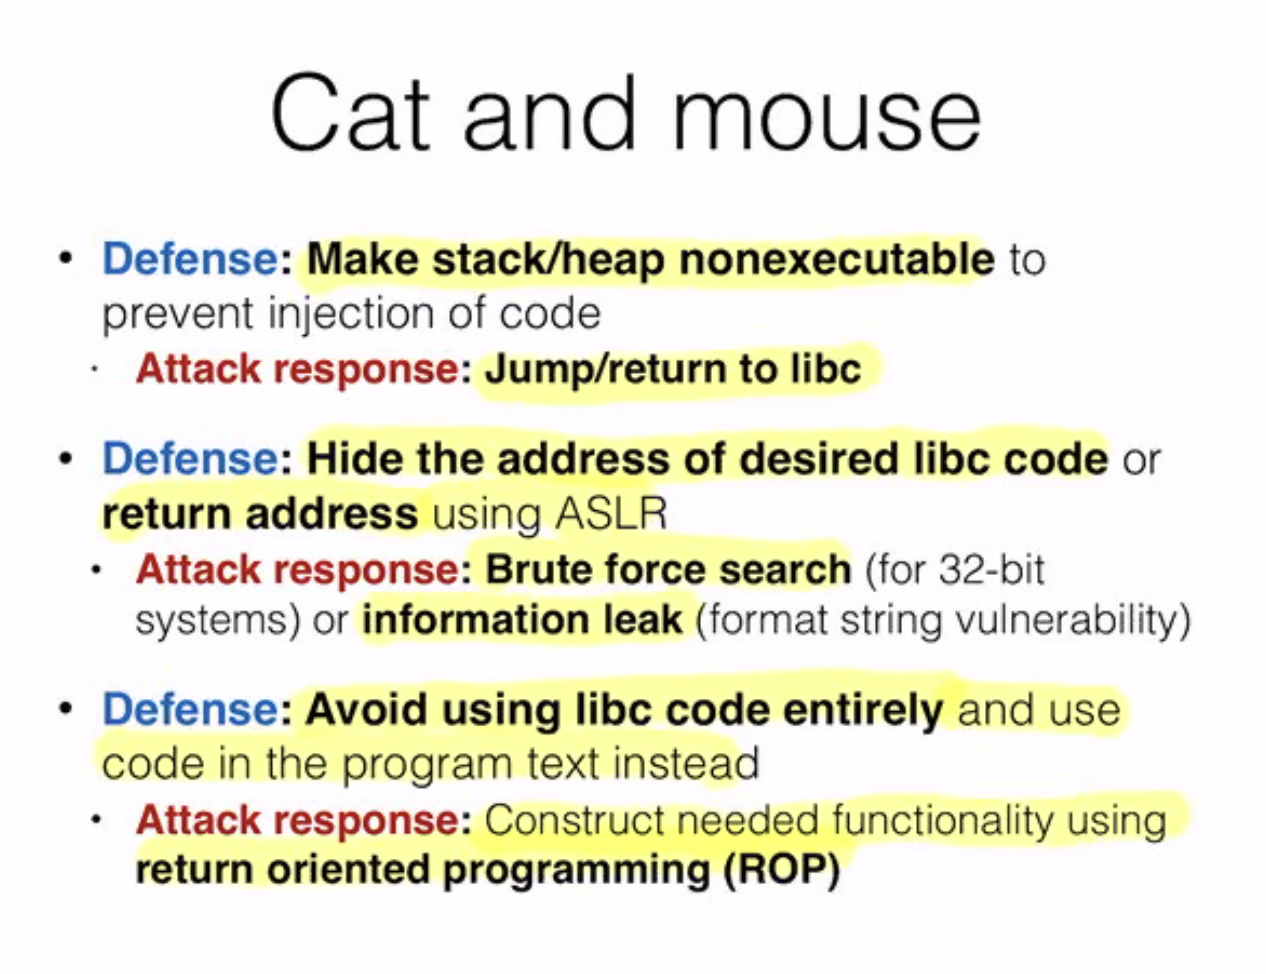
\includegraphics[scale = 0.4]{catmouse}
\end{center}

\section*{Return oriented Programming}
First introduced by Hovav Shacham in 2007, the idea is: rather than use a single libc function to run the shellcode, we string together pieces of existing code called gadgets to do it. Intuitively, we need to find the gadgets we need, and we need a mechanism to string them together
\subsection*{Gadgets}
Gadgets are instruction groups that end with \emph{ret}:
\begin{figure}[H]
\begin{center}
\begin{subfigure}[H]{0.2\linewidth}
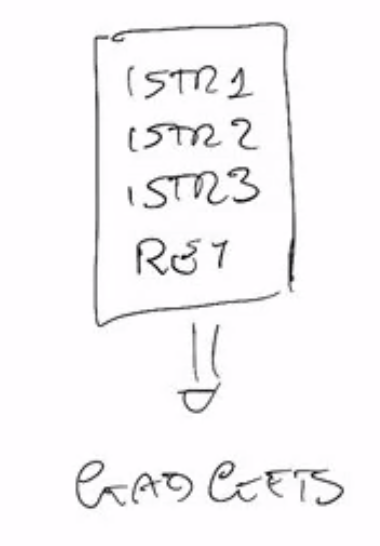
\includegraphics[width=\linewidth]{gadget}
\end{subfigure}
\begin{subfigure}[H]{0.5\linewidth}
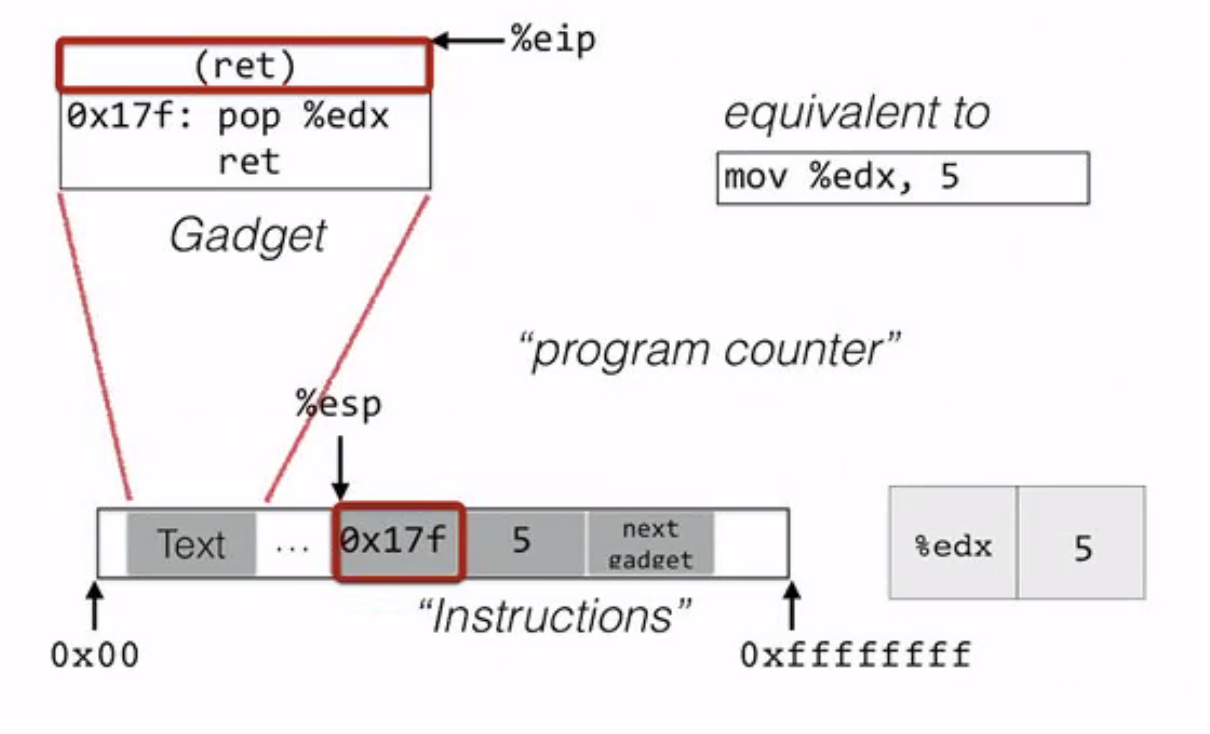
\includegraphics[width=\linewidth]{gadex}
\end{subfigure}%
\end{center}
\end{figure}
The memory structure that we're using is still the stack, which is also where we're loading our code.\begin{itemize}
\item \%esp serves as program counter
\item \emph{gadgets} are invoked via \emph{ret} instruction
\item \emph{multiple gadgets} are linked with each others using \emph{ret} instructions
\item \emph{gadgets} get their arguments via \emph{pop, peek etc.}
\end{itemize}
In this example we're trying to find an applicable instruction equivalent to \emph{mov \%edx, 5}, being: \emph{pop \%edx ret}.

\subsection*{So how do I actually find gadgets?}
One approach would be an automated search of the target binary for gadgets. This technique works by looking for \emph{ret} instructions, by working backwards.
\subsection*{Are these gadgets actually enough to do anything interesting?}
Yes, Shacham found that with significant codebases (such as libc) gadgets are \emph{Turing complete} meaning they're theoretically capable of solving any computational problem. Scwartz, in 2011, automated the gadget shellcode creation process (ROP compiler), without needing Turing completeness.\\\\
In CISC there is a degree of variability in the length of instruction (which is not present in ARM for example since it's a RISC)(RISC instruction lengths are fixed) which provides an extensive degree of freedom to exploits gadgets. This particular aspect is called dense Instruction Set.
\begin{figure}[H]
\begin{subfigure}[H]{0.4\linewidth}
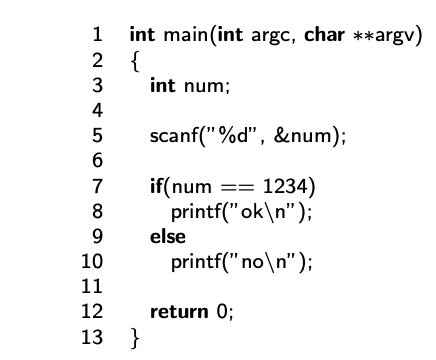
\includegraphics[width=\linewidth]{b1}
\end{subfigure}
\begin{subfigure}[H]{0.5\linewidth}
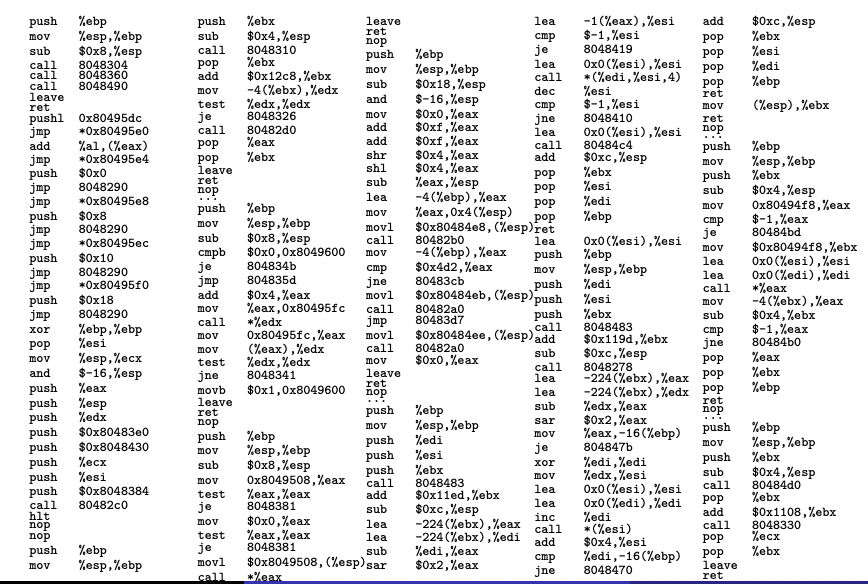
\includegraphics[width=\linewidth]{b2}
\end{subfigure}%
\end{figure}
With a simple program like this, we can extract a gigantic amount of instruction.
\section*{Hacking Blind}
Berkley students managed to attack victim server via a socket, which has all the defence mechanisms we have previously seen enabled, namely ASLR, canary and DEP. The attack happens based on a socket and a linux 64 bit server, via buffer overflow. The exploitation is based on the \emph{write} function:\begin{center}
\emph{write(SD, [buffer], length)}\\
SD is socket descriptor
\end{center}
Utilising a flaw in the \emph{write} function the attacker is able to copy the buffer portion of memory
\begin{center}
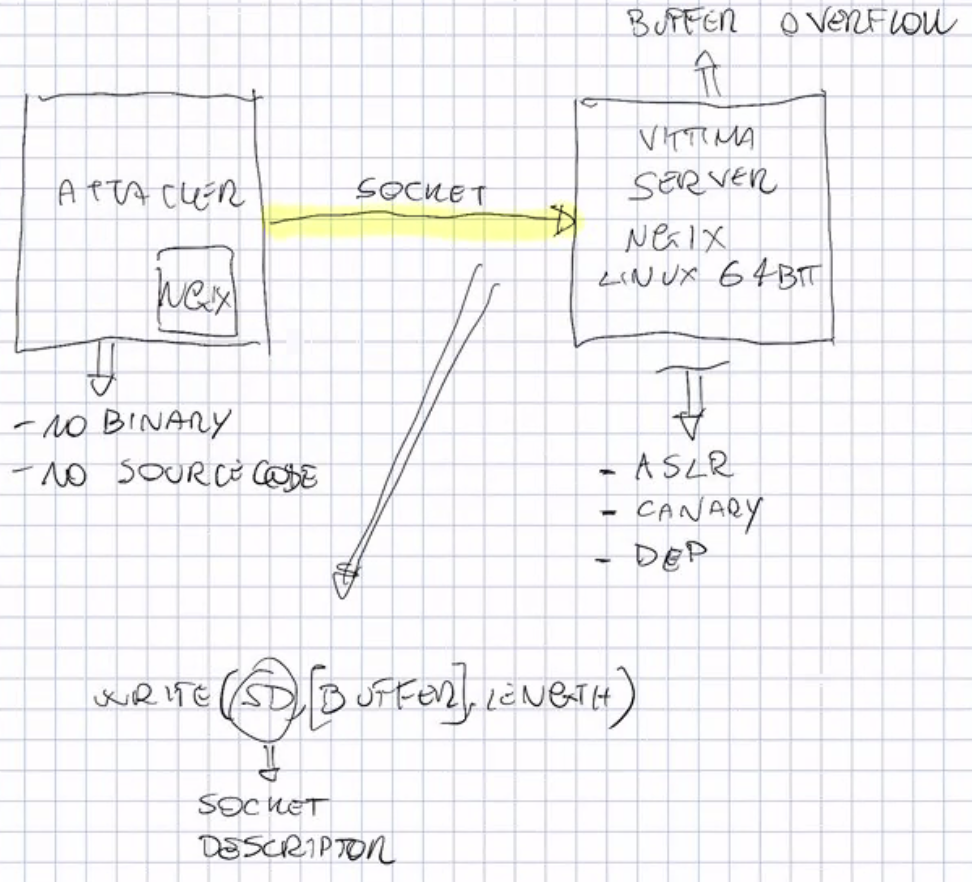
\includegraphics[scale = 0.5]{socket}
\end{center}
A fully automated attack based on this exploit yields a shell in under 4000 requests (20 minutes) against a modern system. 
\subsection*{Techniques needed}
\begin{enumerate}
\item Generalised stack reading: \\
the possibility to read the stack in its entirety, used to leak the canaries (replace them with the correct values), and to defeat the ASLR (if I am able to read the stack, I am also able to read the location of the program).\\
The canary attack these students did is based on the fact that when a thread crashes on a server, only the thread is reset and not the entire system, and therefore the canary value remains the same. The attacker can progressively guess byte per byte the value of the canary. In this example the canary is of size 4 bytes, but on 64 bits system the canary is of size 8 bytes.
\begin{center}
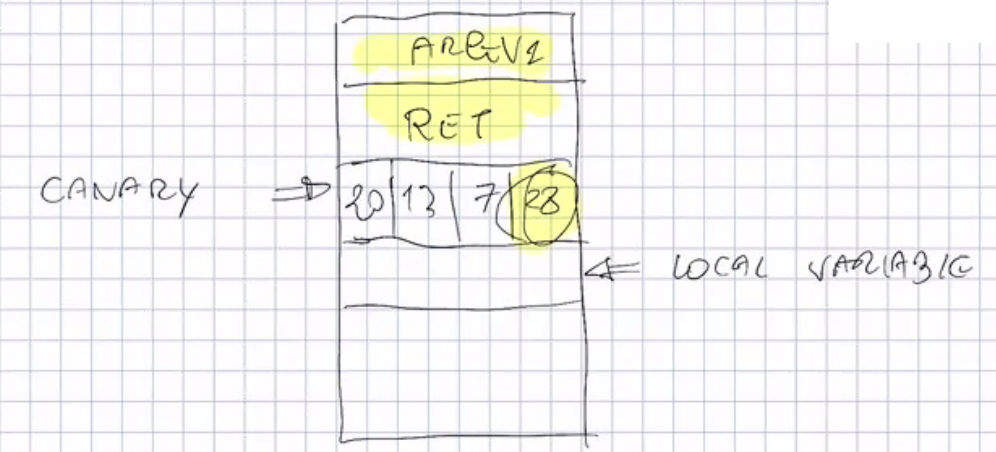
\includegraphics[scale = 0.5]{cattack}
\end{center}
To guess the canary we try every value from \emph{0 to 256} every byte, when the thread crashes we proceed with the next value, if the custom value doesn't invoke a crash, we found our value. Using this technique we can also guess the value of the return address.

\item Blind ROP: this technique remotely locates ROP gadgets (write functions)\\
The goal is to find enough gadgets to invoke \emph{write}. If we manage to do this, the binary can be dumped from memory to network finding even more gadgets in the process. As previously mentioned, the \emph{write} system call takes 3 arguments: a socket, a buffer and a length. These are passed in \emph{rdi, rsi, rdx} registers, and the system call is stored in the \emph{rax} register. The following gadgets are therefore needed:
\begin{center}
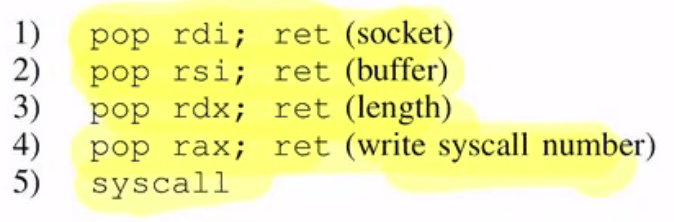
\includegraphics[scale = 0.5]{gadg}
\end{center}
\subsection*{But how do we find these gadgets?}
\emph{pop rdi, rsi, rdx} are manageable, \emph{pop rax and syscall} are the problematic functions, syscall is almost never called since this is usually done through libraries.\\
To effectively find gadgets, we modify progressively the return address, sorting them into crash gadgets, which cause the socket to crash, non-crash gadgets, which produce an arbitrary effect. 
\begin{center}
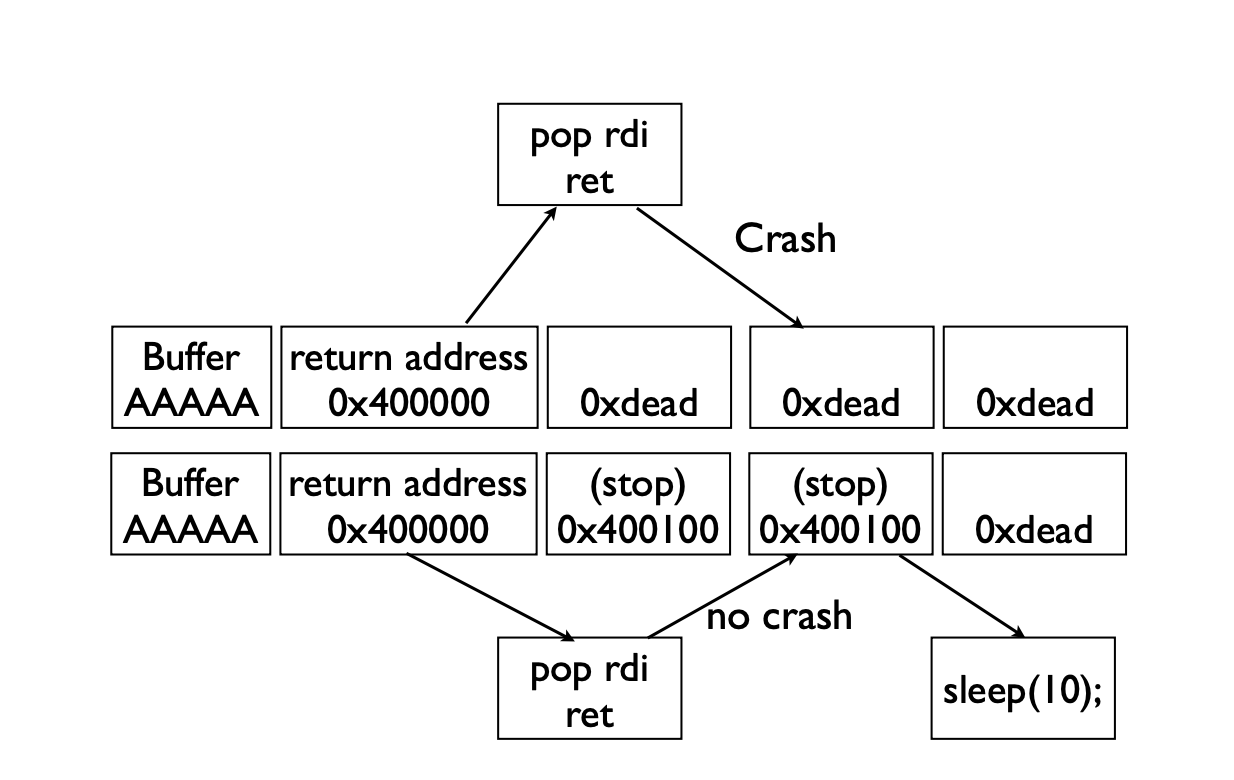
\includegraphics[scale = 0.5]{cgadg}
\end{center}
We further elaborate on non-crash gadgets, implementing probes, traps and stops. If the gadget produce the effect we want the stop is invoked and the gadget is selected.
\begin{center}
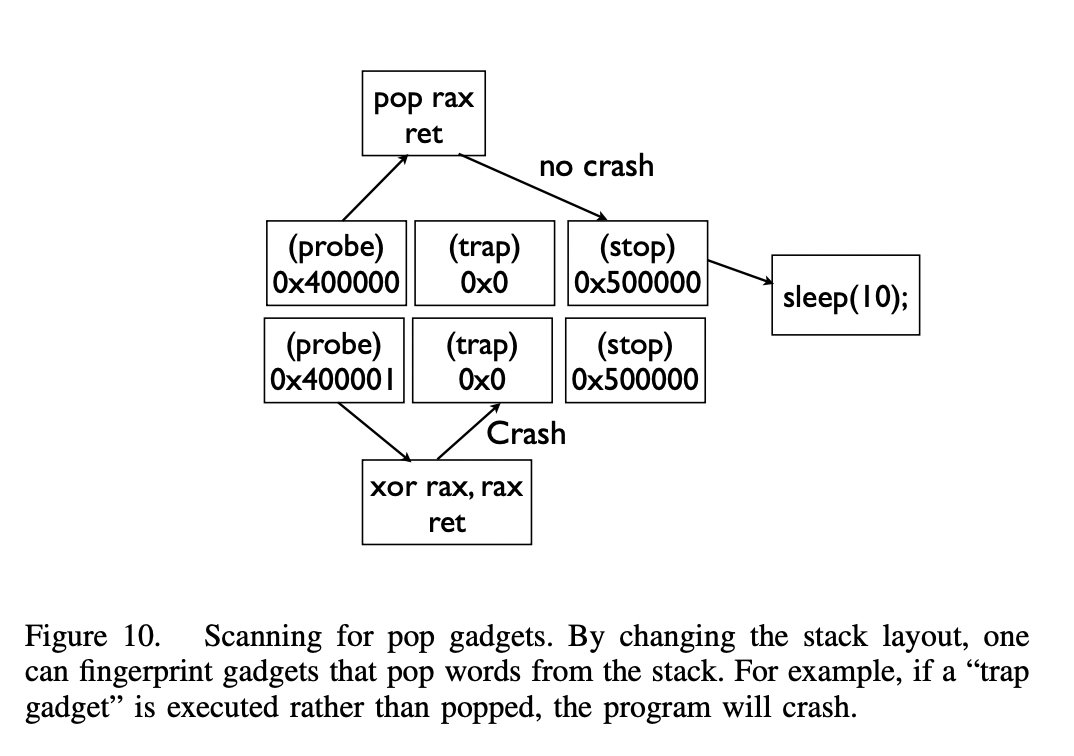
\includegraphics[scale = 0.4]{popstore}
\end{center}
\end{enumerate}
To call functions the PLT (static loader table) and GOT (populated by the dynamic linker) tables are used at runtime to find libraries.
\begin{center}
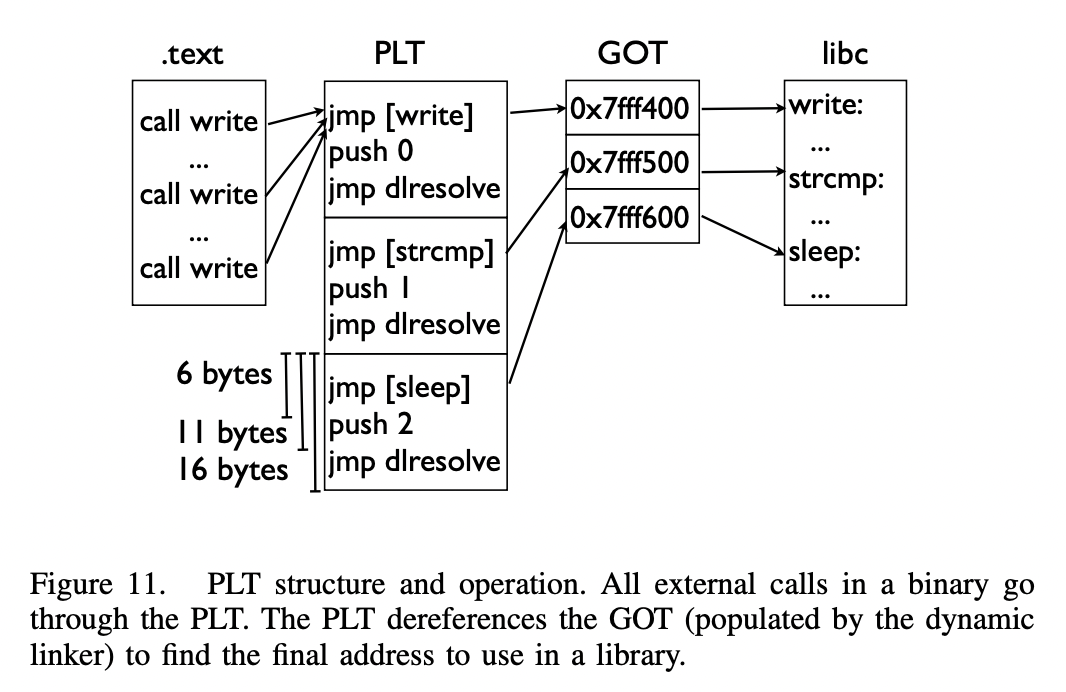
\includegraphics[scale = 0.4]{plt}
\end{center}
We have seen that memory safety and type safety solve most of the memory errors, \emph{control flow integrity} is the last passive defence mechanism we see.



\section*{Control flow integrity}
CFI aims to defend a program by observing the program's behaviour, if the program is not doing what we expect it to do, it might be compromised. To do this we need to define an \textbf{expected behaviour}, create mechanisms which let us \textbf{detect deviations from expectations effectively}, implement policies which \textbf{prevent compromise of the detector}
\subsection*{How efficient is CFI ?}
Classic CFI imposes a 16\% overhead on average, 45\% in the worst cases, it works on arbitrary executables, and is not modular.\\
Modular CFI imposes a 5\% overhead on average, and 12\%in the worst cases, it works only in C (part of the LLVM, source code), and is modular, with separate compilation routines
\subsection*{How secure is CFI actually?}
MFI can eliminate 95\% of ROP gadgets on x86-64 versions of SPEC2006 benchmark suites. Average indirect-target reduction is of $>99\%$, meaning that the percentage of possible targets of indirect jumps is almost completely ruled out.

\subsection*{Randomness and immutability of the detector} 
A degree of randomness and immutability is added to the detector to avoid compromise


\subsection*{Control flow graph | CFG} to define expected behaviour.
One way we can do this is by utilising \textbf{call graphs}. The aim is to represent all the possible combinations of function calls to other functions
\begin{center}
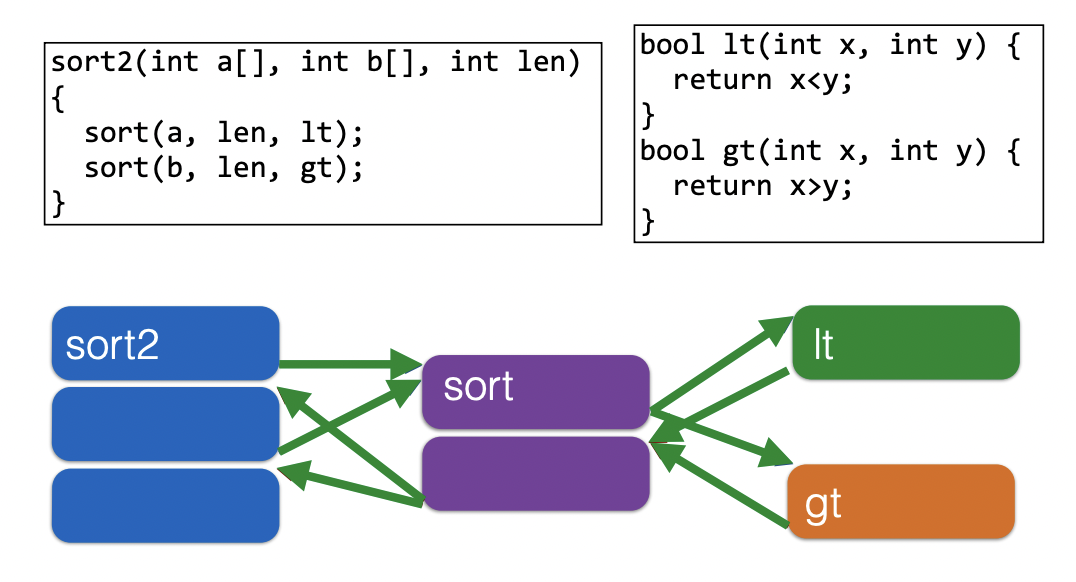
\includegraphics[scale = 0.4]{cfi}\\
\emph{example of a function which sorts by calling 2 distinct functions}
\end{center}
The code is broken up into \textbf{basic blocks}, \textbf{calls} are distinguished from \textbf{returns.}
We compute call/returns CFG in advance, during the compilation or from the binary. We monitor the control flow of the program and ensure that it only follows paths allowed by the CFG.\\\\
Note that calls can be divided into direct calls and indirect calls: \emph{direct calls jump to fixed addresses}, the target address cannot be changed; \emph{indirect calls are calculated at run-time}, the value of the target address cannot be calculated beforehand, these are \emph{jmp, call, ret}.\\
We only need to monitor \textbf{indirect calls}, direct calls need not be monitored since an attacker cannot change a fixed address.
\begin{figure}[H]
\begin{subfigure}[H]{0.5\linewidth}
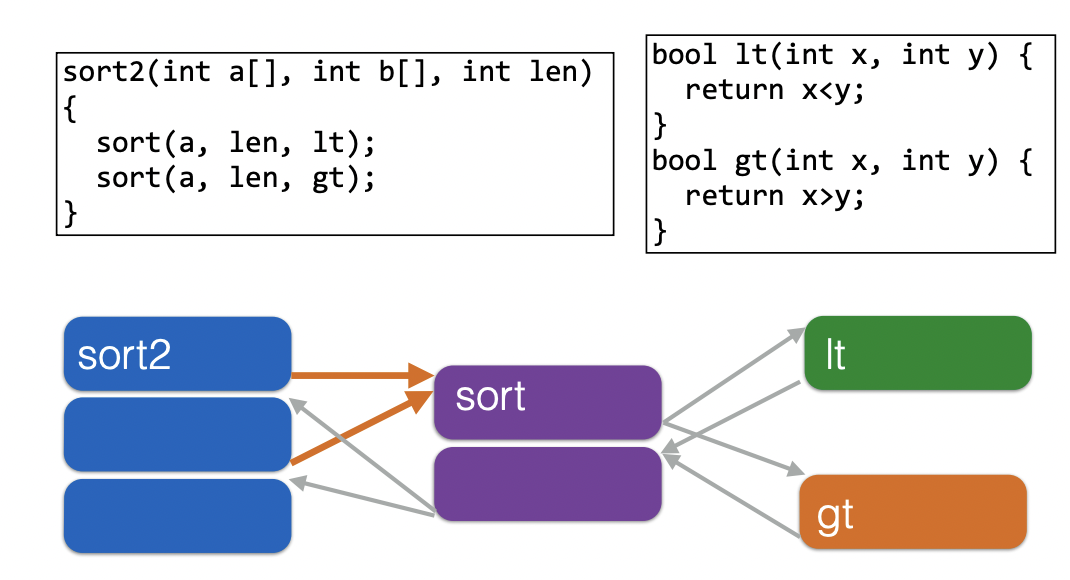
\includegraphics[width=\linewidth]{cfi2}
\emph{direct calls always have the same target}
\end{subfigure}
\begin{subfigure}[H]{0.5\linewidth}
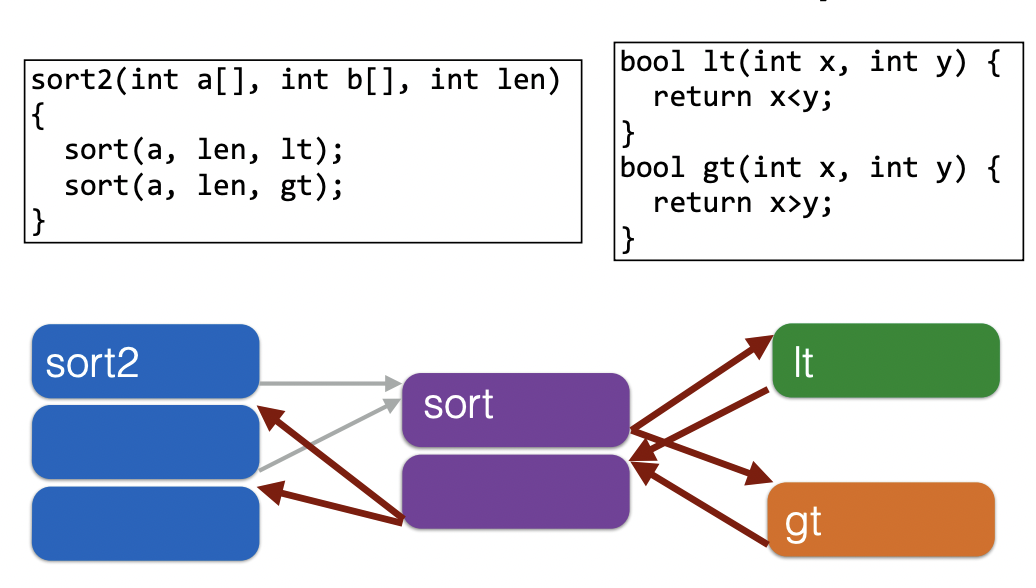
\includegraphics[width=\linewidth]{cfi3}
\emph{indirect transfers do not}
\end{subfigure}%
\end{figure}

\subsection*{In-line reference monitor | IRM} 
IRM is used to detect deviations from expectations, it works by introducing control methods inside the program (in binary or inside the program) (program transformation). More particularly we utilise labels, determined by the CFG:\begin{itemize}
\item insert a label just before the target address of an indirect transfer
\item insert code to check the label of the target at each indirect transfer\\
If the label does not match, we abort the execution
\end{itemize}
\begin{center}
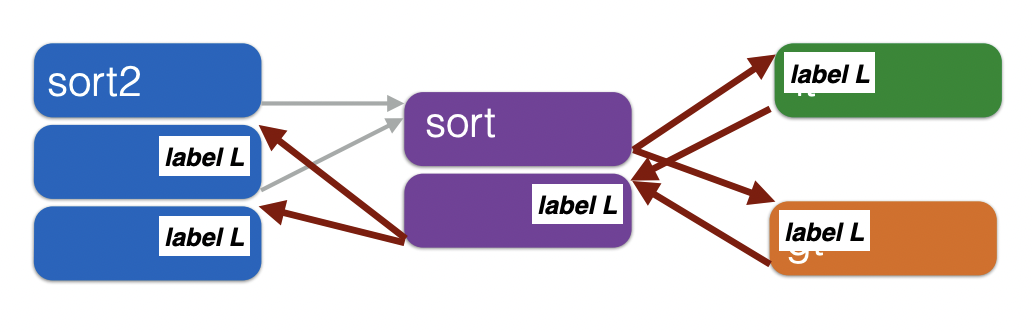
\includegraphics[scale = 0.4]{labels}
\end{center}
If for example an attacker manages to hijack the control flow of the program, when he tries to access a system call the jump is denied, since it's not validated by the CFG.
\begin{center}
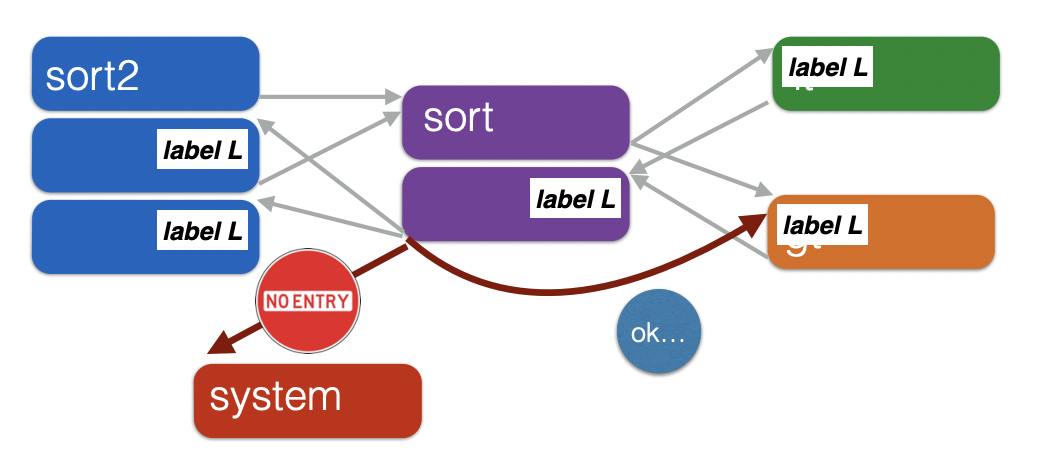
\includegraphics[scale = 0.4]{labels2}
\end{center}
We can further improve simple labelling by introducing \textbf{detailed labelling}
\begin{center}
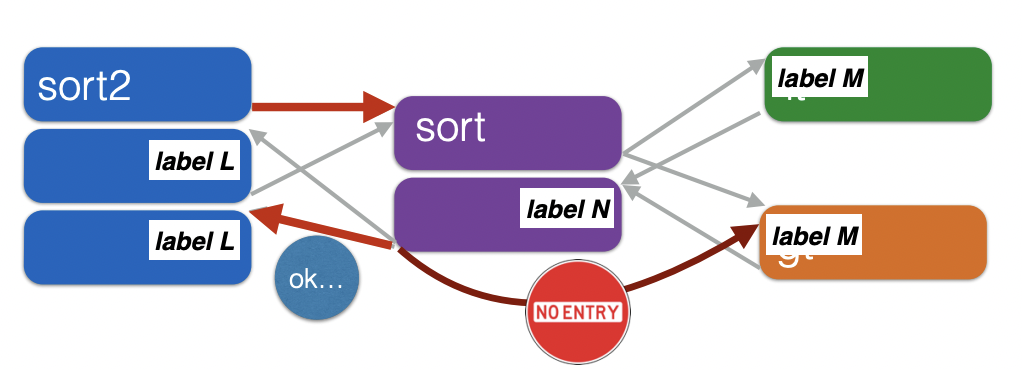
\includegraphics[scale = 0.4]{labels3}
\end{center}
\begin{itemize}
\item return sites from calls to \emph{sort} must share a label $L$
\item call targets $gt$ and $lt$ must share a label $M$
\item remaining labels are unconstrained $N$
\end{itemize} 
So how can we defeat CFI?
\begin{itemize}
\item inject code that has a \emph{legal label}\\
- won't work since we assume non-executable data
\item modify code labels to allow a desired control flow\\
- won't work since the code is immutable
\item modify the stack during a check\\
- won't work since the attacker cannot change register 
\end{itemize}
\subsection*{CFI assurances}
CFI defeats control flow-modifying attack such as remote code injections, ROP/return to libc, etc.
\begin{itemize}
\item It cannot defeat attacks based on manipulation of control flow that is allowed by the labels/graph, these are called \textbf{mimicry attack}. These attack mimic a valid control flow, bypassing detection.\item It cannot defeat data leaks or corruptions, heartbleed cannot be prevented, nor the \emph{authenticated} overflow. In simpler terms, attacks based on the modification of attributes and variables are not preventable using CFI, such as:
\begin{center}
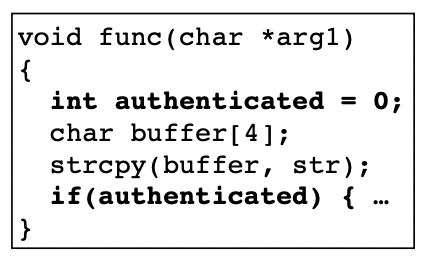
\includegraphics[scale = 0.6]{cfia}
\end{center}
\end{itemize}

\section*{Static Analysis and Dynamic Analysis | persa prima parte}
Analysis can range from static to dynamic, and from automatic to manual. The main advantage of static analysis is that when designed, it's fast to execute; the downside is that the precision is not that great, potentially leading to false positives.  Dynamic analysis is more precise than static analysis, and is done by actually executing the program and closely monitoring the execution. The downside of dynamic analysis is that only a single input can be verified at a time, making it slow (as compared to static)
\begin{center}
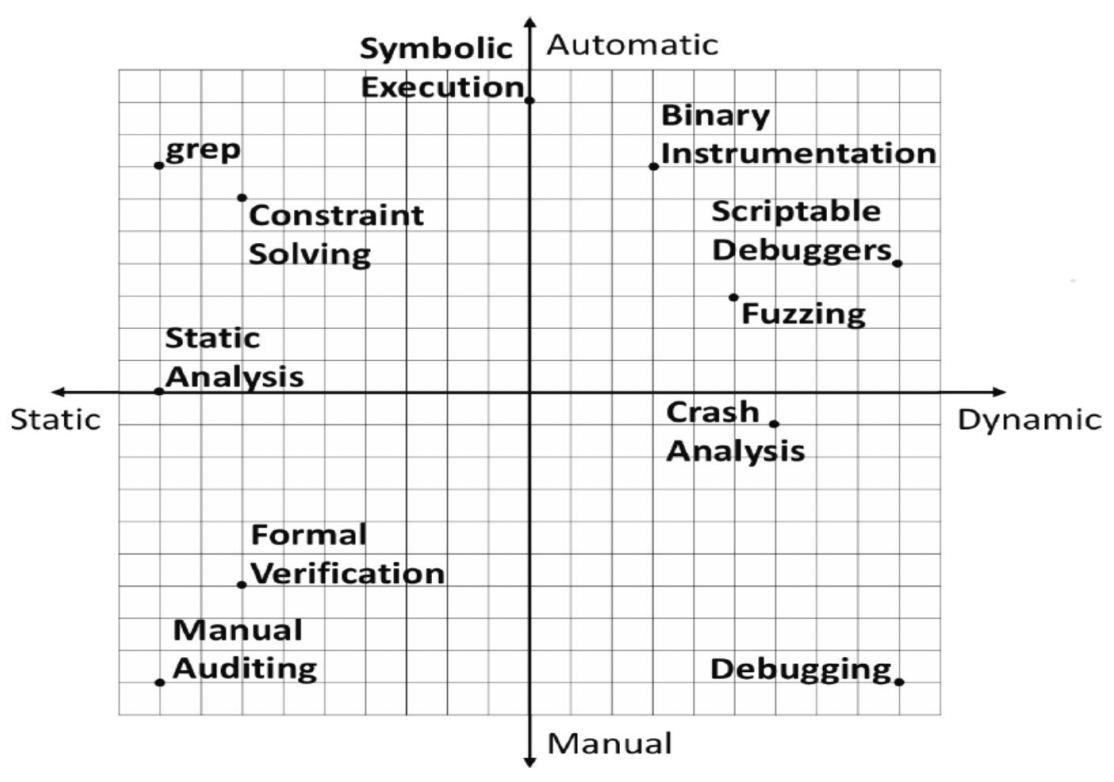
\includegraphics[scale = 0.6]{dov}\\
\emph{main vulnerability detection techniques}
\end{center}
The most common technique is debugging, monitoring the system execution looking for bugs and flaws. Symbolic execution is an example of testing that can be done both statically, and dynamically. Crash analysis aims to crash the program intentionally, and analyse the system's dump (root cause analysis).
\subsection*{Detection of the vulnerability}
The aim of this process is to detect the presence of vulnerabilities in the code during the stages of development, testing, and maintenance.
\subsection*{Soundness and completess}
While considering the tools available to us we need to consider the trade-off between \emph{soundness} and \emph{completeness}.\\

A detection technique is considered \textbf{sound} if for a given category, it can correctly conclude that a given program or system has or hasn't vulnerabilities (per una data categoria è in grado di dirmi se il programma è sicuro | eg. niente bof).\\
An unsound detection technique, on the other hand, may have \textbf{false negatives}, meaning that actual vulnerabilities may slip through the tool's detection techniques.\\
Achieving soundness requires a consideration based on all execution of a program. This can be done by static checking of the program code, and building up an abstraction of the program execution. Using this abstraction we aim to execute the program in all its possible permutations.\\


A detection technique is \textbf{complete} for a given category if any vulnerability if finds is an actual vulnerability. By contrast and incomplete detection may have \textbf{false positives}, it may therefore detect issues which aren't actually vulnerabilities.\\
Achieving completeness can be done by executing the program that show the vulnerability, this analysis technique should provide concrete inputs that triggers a vulnerability. Software testing is a way a developer can achieve completeness, by writing test cases with concrete inputs, and specific checks for the outputs\\\\
In the real world techniques are mixed and used concurrently to analyse the program, employing both static and dynamic analysis to achieve a good trade-off between soundness and completeness. An hypothetical tool may be able to achieve both soundness and completeness, unfortunately such a tool doesn't exist, so we try to balance in the best way we can.

\subsection*{Static analysis and Symbolic execution}
Static analysis is any offline computation that inspects the code and produces results based on the quality of the code. This can be applied both for source code and binary code. 
Techniques include regular expressions, classic compiler flow analyses or some combination of these. It is important to note that static analysis does not have to use symbolic execution (input non concreti, ma associati a simboli). \\

Symbolic execution is a specific kind of off-line computation that computes some approximation of what the program actually does by constructing formulas representing the program state at various points. It is called symbolic because the approximation is usually based on some formula involving program variables and constraints on their values.\\
\subsection*{Symbolic execution}
Testing is a technique widely used in software engineering and works by utilising assertions such as \begin{center}
$assert(f(3) == 5)$\end{center}
This technique is \emph{complete}, meaning that a bug found is a real bug, but \emph{not sound} since each test can only explore one possibility.\\
Symbolic execution generalises testing, the aim is to make employ a "more sound" technique that testing. Symbolic execution allows the implementation of unknown symbolic variables $\alpha$ in an evaluation such as\begin{center}
$y = a; assert(f(y) == 2* y-1)$\\
\noindent\rule{8cm}{0.4pt}
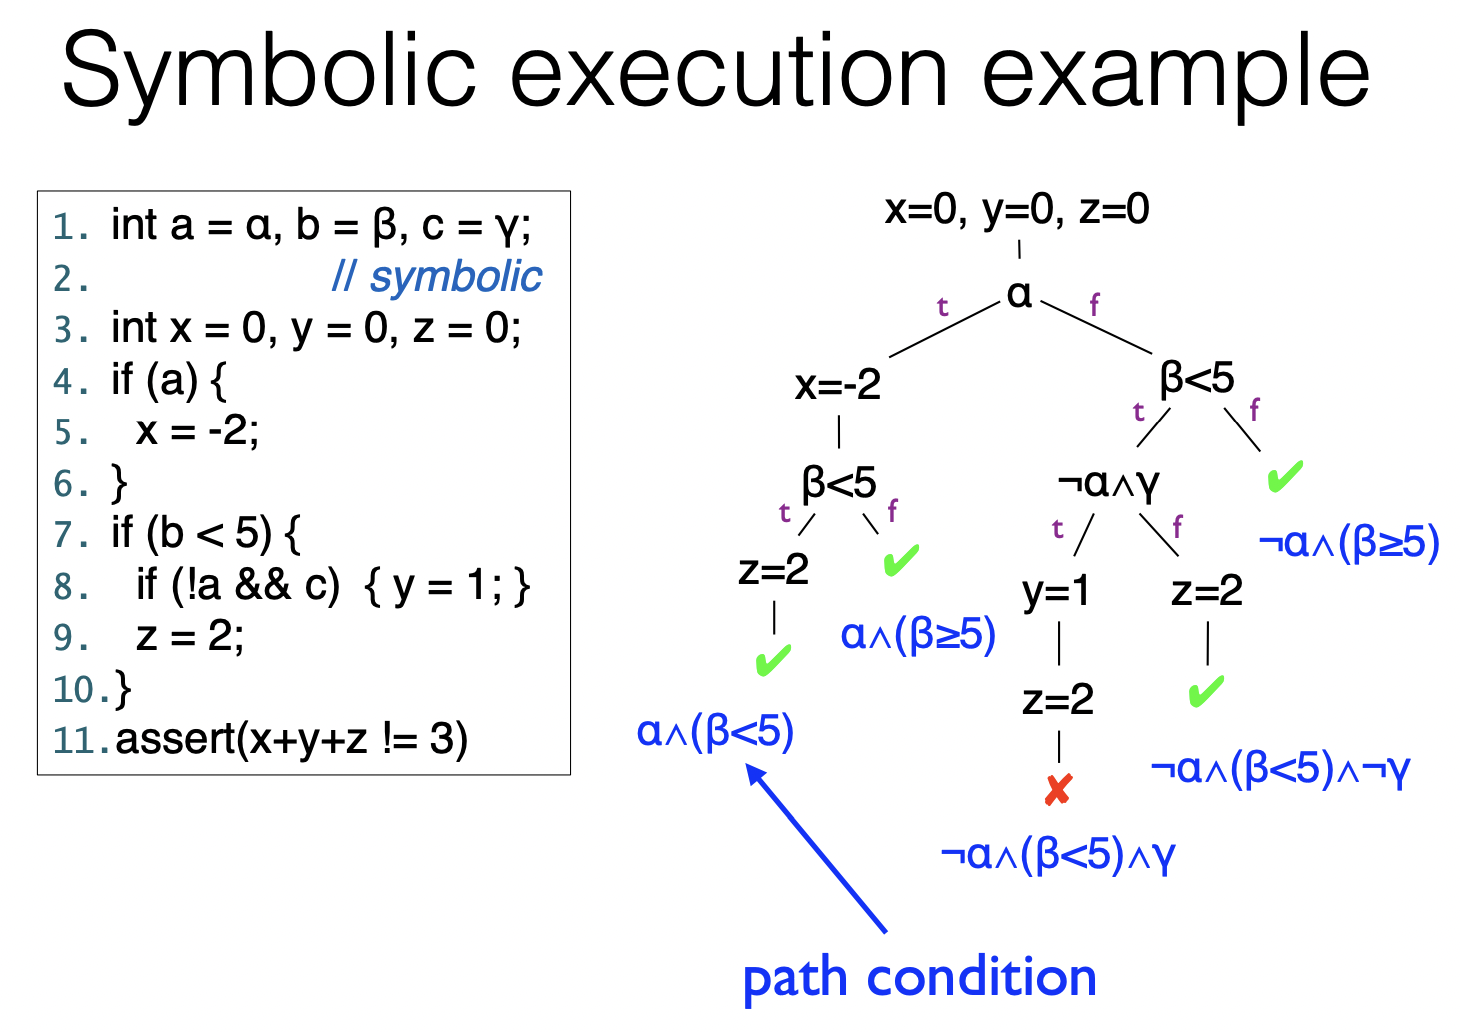
\includegraphics[scale = 0.4]{dov2}
\end{center}
The path condition represents the input condition needed to reach a specific outcome. Each path condition can be used to create an actual input (usually done by the constraint solver). Soundness is partially achieved since we're able to verify for a number permutations of inputs. Each symbolic execution path stands for many actual program runs, as many concrete run under symbolic execution paths. We cover a lot more of the program's execution space than testing. \\
Static execution can therefore be viewed as static analysis which is complete, but not sounds; it is path, flow and context sensitive.
\subsubsection*{A bit of history}
First implemented in the 70s, it didn't take off right away since symbolic execution can be quite computer intensive due to the high number of possible program paths, need to query solve a lot to decide which paths are feasible and which assertions could be false. Computer were slower and smaller, not equipped with a lot of processing power. Nowadays, however, computer are faster and bigger, and symbolic execution is making a comeback also due to better algorithms and SMT/SAT (satisfiability modulo theories) solver, which can solve large instances very quickly
\subsection*{Symbolic variables}
Symbolic variables are an extensions of the language to support expressions $e$ to include symbolic variables, representing unknowns (but supported by the program itself)
\begin{center}
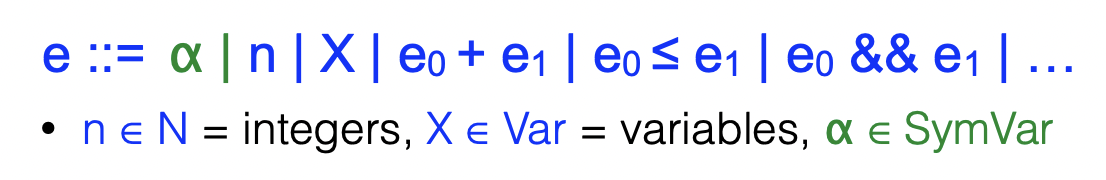
\includegraphics[scale = 0.4]{dov3}
\end{center}
Symbolic variables are introduced when reading inputs, particularly when using \emph{nmap, read, write, fgets etc.} If a bug is found, we can safely extract the input that produces the error.
Furthermore we need to make or modify a language interpreter to be able to compute symbolically. normally a program's variables contain values, we modify them by also making sure they support \emph{symbolic expressions}.
\begin{center}
$5, "hello" \rightarrow \alpha + 5, hello + \alpha etc.$
\end{center}
Consideriamo il seguente programma:
\begin{center}
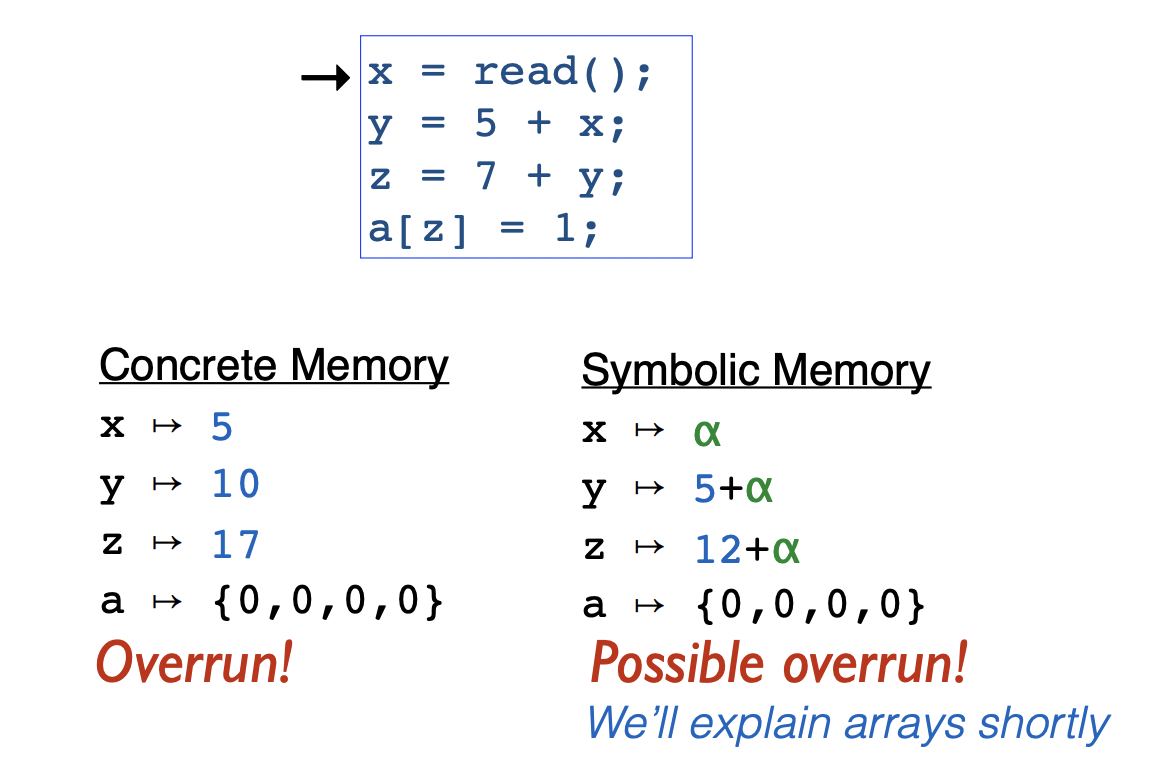
\includegraphics[scale = 0.4]{dov4}\\
\emph{the overrun comes from the fact that z has a value which exceed the array bounds of a}
\end{center}
But in symbolic memory the value of $\alpha$ \emph{can} exceed the bounds, but not necessarily

\subsection*{Path conditions}
As previously said, path conditions are necessary conditions on inputs for reaching the target location is disjunction of all abstract path conditions. More specifically in programming a path condition diverges from another when an $if$ is encountered, for example:
\begin{center}
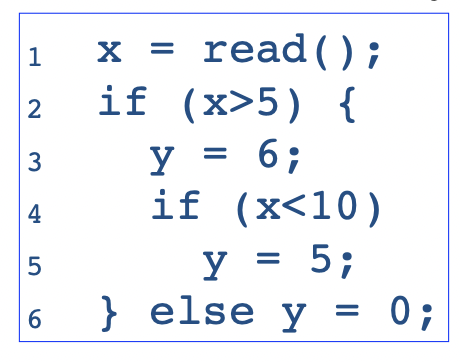
\includegraphics[scale = 0.4]{dov5}
\end{center}
We represent the influence of symbolic values on the current path using a path condition $\pi$, particularly:\begin{itemize}
\item line 3 reached when $\alpha > 5$
\item line 5 reached when $\alpha > 5$ and $\alpha < 10$
\item line 6 reached when $\alpha \geq 5$
\end{itemize}
Not all path are reachable, particularly we talk about \emph{path feasibility} when we talk about whether a path is feasible 
\begin{itemize}
\item line 3 reached when $\pi = \alpha > 5$, solution to which can be $\alpha = 6$
\item line 5 reached when $\pi = \alpha > 5$ and $\alpha < 10$, but this is not satisfiable, the value of $\alpha$ cannot be both bigger than 5 and smaller than 3
\item line 6 reached when $\pi = \alpha \geq 5$, solution to which can be $\alpha = 2$
\end{itemize}
\subsection*{Paths and assertions}
\begin{center}
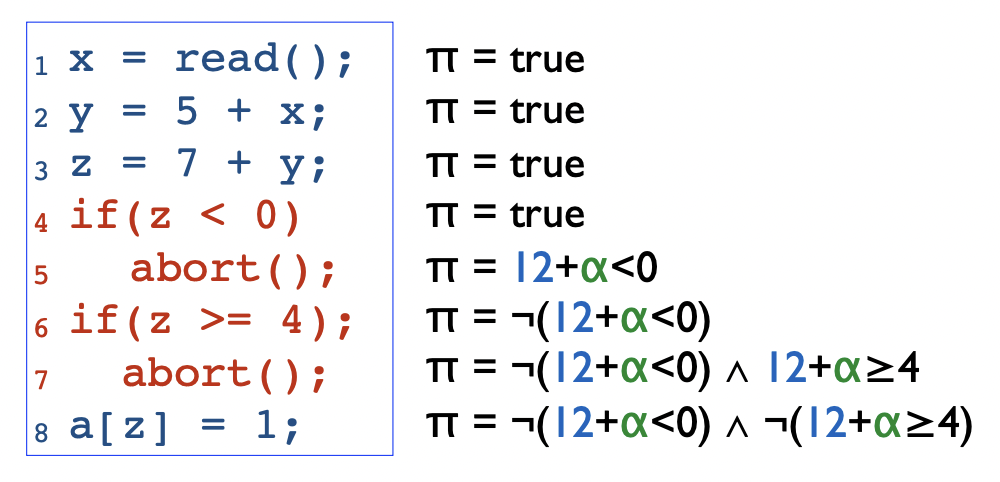
\includegraphics[scale = 0.4]{dov6}
\end{center}
Assertions like array bounds checks are conditionals, can therefore verifiable. A security analyst can for example check the value of the index of an array during testing. If there is a feasible path leading to the aborts, we can deduce that the program has a security flaw/bug, if there are no feasible aborts, the program is safe.\begin{itemize}
\item to reach the line 5: \begin{center}
$\pi = 7+5+\alpha= 12+\alpha \rightarrow \pi = 12+ \alpha < 0$
\end{center}
\item to reach the line 7 abort: \begin{center}
negate the line 4 condition, add the line 6 condiiton:\\
$\pi = \lnot(12+\alpha < 0) \land(12+\alpha \geq 4)$
\end{center}
\end{itemize}
We look for path infeasibility to guarantee that there are no buffer overflow.
\subsection*{Forking execution}
Symbolic executors can fork at branching points, which happen when there are solutions to both the path conditions and its negation. How can we systematically explore both directions?
\begin{itemize}
\item check feasability during execution and queue feasible path for later consideration
\item concolic execution: run the program to completion, then generate new inputs by changing the path condition (esecuzione concreta del programma su dati input, con l'aggiunta dell'esecuzione simbolica)
\end{itemize}
To explore all possible paths we follow the execution algorithm:
\begin{center}
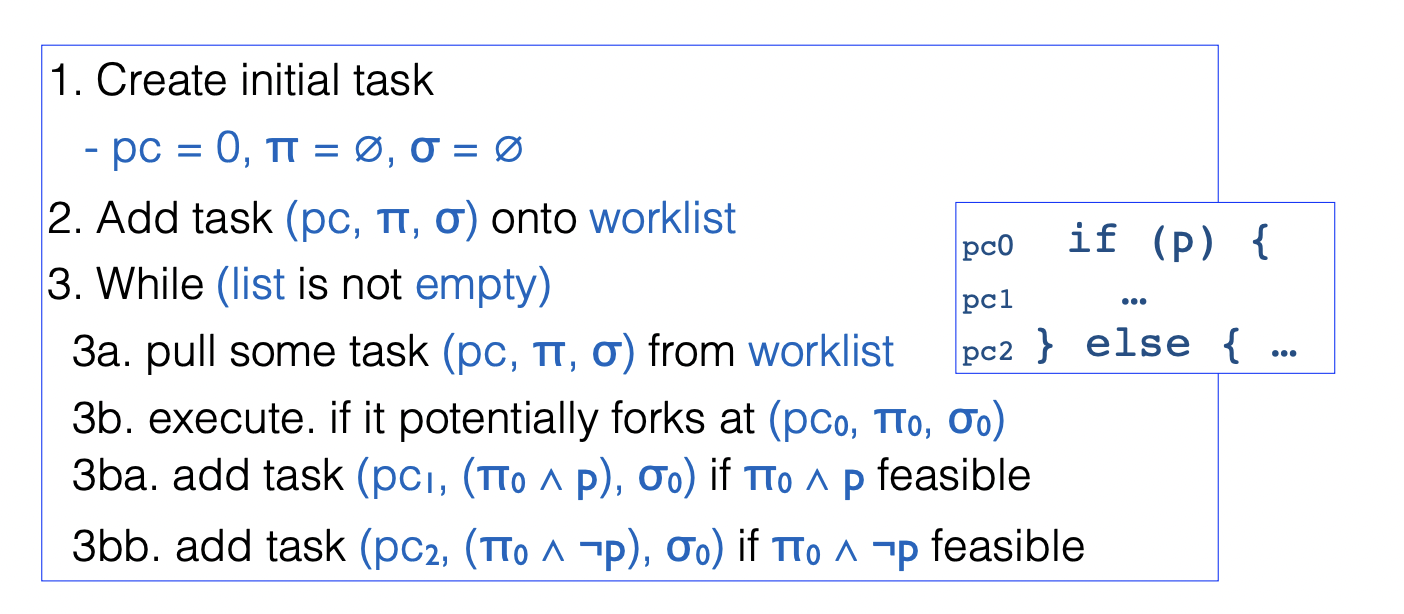
\includegraphics[scale = 0.4]{dov7}
\end{center}
this algorithm is based on a basic depth-search of a graph
\subsection*{Libraries and native code}
At some point symbolic execution will reach the edges of a program such as libraries, systems or assembly code calls. An example can be the libc, which is insanely complicated, way too complicated for symbolic execution which can easily get stuck in it. We can introduce a simpler version of libc, for example newlib.

\subsection*{Concolic execution | Dynamic symbolic execution}
Instead of running the symblic execution in a static way, we instrument the program to do symbolic execution as the program runs, initially the program considers concrete states (which could be randomly generated) to determine initial paths. \\
Each time a branch path is encountered, the expression is saved inside a \emph{shadow path memory}, which are then explored one path at a time, from start to finish. The next path can be determined by negating some element of the last path conditions.\\
Concolic execution makes it really easy to concretise inputs, by replacing symbolic variables with concrete values that satisfy the path condition.

\section*{Search and SMT}
Symbolic execution is appealingly simple and useful, but it's computationally expensive. Let's see how the effective use of symbolic execution boils down to a kind of search, and take a moment to see how its feasibility at all has been aided by the rise of SMT solvers. Basically the practical use of symbolic execution boils down to \begin{itemize}
\item searching for the paths
\item solving the symbolic execution for these paths using SMT solvers while accounting for feasibility
\end{itemize}
One of the first thing to note is that we cannot run symbolic execution to exhausting, since this would quickly generate a exponential number of branches
\begin{center}
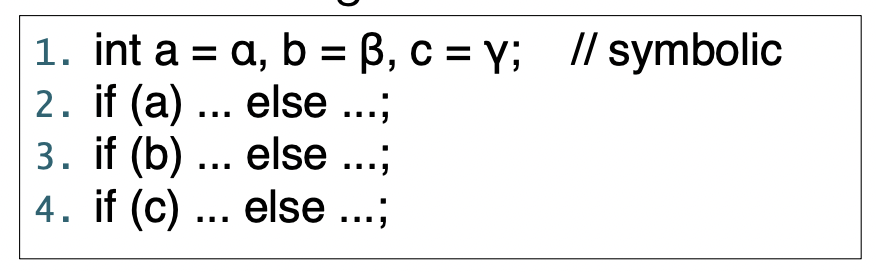
\includegraphics[scale = 0.4]{pc1}\\
\emph{3 variables, 8 program paths}\\
\end{center}
And loops are even worse
\begin{center}
\includegraphics[scale = 0.4]{pc2}\\
\emph{potentially $2^{31}$ paths}
\end{center}
Concolic execution, as opposed to static analysis, doesn't terminate before considering all possible program runs. Static execution approximates multiple loop executions, assuming all branches or a number of loop iterations are feasible; this however can lead to false alarms. Concolic execution of the other hand aims to be more precise, granting more completeness.
\subsection*{Basic symbolic execution}
\emph{So how do we actually look for the possible paths?}\\
Simply, using search algorithms, in particular
\begin{itemize}
\item Depth-first search (DFS) using a stack as work-list
\item Breadth-first search (BFS) using a queue as work-list
\end{itemize}
Potential drawbacks to this approach are that searches cannot be guided by any higher level knowledge (getting stuck in loops, path explosion etc.), moreover \emph{DFS} can easily get stuck in parts of programs, making \emph{BFS} the better choice between the two.

\subsection*{Advanced symbolic execution}
As we have seen DFS and BFS are not optimal solutions, let's focus on prioritising searches, trying to steer searching towards paths more likely to contain assertions failures, and imposing a time limit on execution.\\
To this end, let's think of a program execution as a DAG in which

\begin{center}
$Nodes = program states$\\
$Edges(n_1, n_2) =$ transition from state $n_1$ to $n_2$
\end{center}
Intuitively we need a new graph exploration algorithm.

\subsection*{Randomness}
Since we don't know a priori which path to take, we add a degree of randomness,  we start by taking a concrete path, then executing a symbolic execution, randomly generating an expression $n$ times, if no effects are detected we move on.
\begin{enumerate}
\item pick next path to explore uniformly at random
\item randomly restart search if we haven't hit anything interesting in a while
\item choose among equal priority paths at random
\end{enumerate}
The problem with randomness is its non-reproducibility, we cannot reproduce specific execution unless we save the seeds.

\subsection*{Coverage guided heuristics}
Coverage guided heuristics tries to keep a tab on previously visited paths using a score system. We visit statements we haven't seen before (or lowest score)
\begin{itemize}
\item we give a score to each statement based on the number of times it has been seen
\item we pick the next statement to explore based on the lowest score
\end{itemize}
This technique tries to reach everywhere, even in hard to reach parts of the programs. The problem with this approach is that it may never be able to get to a statement if proper precondition not set up.

\subsection*{Generational search}
Generational search is a hybrid of BFS and coverage-guided, this technique aims to increase the level of coverage
\begin{itemize}
\item Generation 0: pick one program at random, run to completion
\item Generation 1: take paths from $gen_0$, negate one branch condition to yield a new prefix, find a solution for this prefix and take the resulting path
\item Generation $n$: branch off again from $gen_{n-1}$
\end{itemize}
Generational search also uses coverage heuristic to pick priority

\subsection*{Combined search}
Combined search aims to run multiple searches with different techniques at the same time alternating between them, it aims to increase parallelisation. The logic is since no-one-size-fits-all solution, we switch between search techniques based on the occasion, selecting occasionally the algorithm.

\section*{SMT solvers}
SMT solvers are the tools we use to solve SATs.\\
SAT problems is translate in propositional formula that is composed by boolean variables connected by boolean operators ($\not, \lor, \rightarrow)$. \begin{itemize}
\item if the formula is satisfiable, there is an assignment that makes the results true, otherwise the formula is \emph{unsat}
\item the solution to the formula are based on the truth table, the solution to which is exponential
\item SAT is an NP-Complete problem
\end{itemize}
\subsection*{Z3 SAT/SMT Solver}
Z3 SAT/SMT is a SAT solver developed by Microsoft
\begin{itemize}
\item an instance is passed to the quantifier-free SMT solver
\item theory reasoner creates a boolean model, which is then tested by the SAT solver
\item if there are conflict clauses, the model is rejected and the theory reasoner tries again
\end{itemize}
The SMT solver then outputs a model which can be further developed, or the expression is deemed UNSAT
\begin{center}
\includegraphics[scale = 0.4]{theory}
\end{center}
Other SMT solvers are Yices by SRI, STP by Vijay Ganesh, CVC3 by NYU
\subsubsection*{A bit of history}
\begin{itemize}
\item SAGE is a concolic executor developed at Microsoft Research which primarily targets bugs in file parsers (JPEG, DOCX, PPT etc.), uses generational search. SAGE is used on production software at MS (500 machines years, 3.4+ billion constrains, 100s of apps, 100s of bugs)
\item KLEE is a symbolic executor for LLVM bitcode, uses $fork()$ to manage multiple states, uses a variety of search strategies, mainly random path + coverage guided
\item Mayhem runs on binaries, uses BFS search and native execution, combines best of symbolic and concolic strategies, and automatically generates exploits when bugs are found
\item Mergepoint extends Mayhen with a technique called veritesting, combining symbolic execution with static analysis. It provides a better balance of time between solver and executor, finding more bugs, and covers more of the program
\end{itemize}

\section*{Fuzzing techniques}
Fuzzing is an alternative to symbolic execution, it's a kind of random testing, its goal is to make sure certain bad things don't happen no matter. Fuzzing is a process which aims to clear the program of crashes, thrown exceptions and non terminations.\\

Fuzzing is not employed on its own but it complements functional testing, normal tests can be a starting point for fuzz tests, which can then be followed up with direct tests.
Fuzzing must be efficient, 
\subsection*{Fuzzing techniques}
There are 3 main types of fuzzing:
\begin{itemize}
\item black box fuzzing\\
the tool knows nothing about the program or its input, it's \emph{easy to use} and get started, but will explore only shallow states unless it gets lucky since it relies on randomly generated inputs
\item grammar based fuzzing\\
the tool generates input formed by specified grammar, it's \emph{more work to use}, to produce the grammar, but can go deeper in the state space. 
\item white box fuzzing\\
the tool generates inputs partially informed by the code of the program being fuzzed, it's \emph{easy to use}, but computationally expensive due to the analysis that has to be done beforehand
\end{itemize}

\subsection*{Fuzzing inputs generation}
We have seeing the types of fuzzing techniques, but how are inputs actually generated?
\begin{itemize}
\item Mutation\\
we take a legal input and mutate it, and using that as input. Legal inputs may be human produced, for example from a grammar or SMT solver query
\item Generational\\
we generate input from scratch, for example from a grammar
\item Combinations\\
we generate initial inputs and mutate them $n$ times to generate new inputs, or we generate mutations according to a grammar
\end{itemize}
There are many ways to generate input and the technique used need not be only one, we can combine together. Fuzzing is different from symbolic execution since it generate inputs without taking code structure into account (there is no logic regarding $if, else, switch$ structures)
 \subsubsection*{But what happens when the program actually crashes?}
 When a crash actually occurs we look for the root cause, and ways to potentially fix them. More explicitly we ask
 \begin{itemize}
 \item is there a way to make the input smaller, and more understandable?
 \item are two or more crashes signalling the same bug, if yes we can correlate them together (vulnerabilities cluster)
 \end{itemize}
 After identifying the root cause we can analyse the crash looking for exploitable vulnerabilities, for example dereferencing $NULLs$ is rarely exploitable, and buffer overruns are often positioned in a different place than the crash. 
 
 \subsection*{Memory errors}
 One of the other aims of fuzzing is looking for memory errors. One of the ways we do this is by compiling the program with an \emph{Address Sanitiser or ASAN}, an instrument that accesses arrays to check for overflows and use after free errors. \\
 After running \emph{ASAN} we continue by fuzzing it, we analyse is the program crashed with an ASAN signalled error, and if that's the case we worry about exploitability.
 
\subsection*{Symbolic execution vs Fuzzing}
\begin{center}
\includegraphics[scale = 0.4]{sf}
\end{center}
In this example we see that symbolic execution clearly wins, since during white-box fuzzing we keep a track of conditions, generating from the is way simpler, in particular in this example the possibility to generate an input that triggers the error is abysmal. \\
To give a sense of the order of magnitudes, white-box fuzzing, as a recent paper as shown, such as \emph{KLEE} is 3000 times slower than native execution, while \emph{angr} is 300,000 times slower. Given these numbers, achieving 100\% is virtually impossible.


\section*{Meltdown \&Spectre}
Meltdown e Spectre sono due attacchi che sfruttano vulnerabilità nei moderni processori, che permettono ad un attaccante di rubare informazioni sensibili su un computer.\\
Normalmente I processori non sono in grado di leggere informazioni in utilizzo da altri processi, tuttavia con Meltdown e Spectre un attaccante è in grado di accedere a tali informazioni.

\subsection*{Meltdown}
Meltdown è un attacco che rompe la divisione tra applicazioni utente e sistema operazioni, permette ad un programma di accede alla memoria, esponendo informazioni sensibili. 

Meltdown permette di leggere un byte in in una qualunque zona di memoria mappata dal processo dell'attaccante, più in particolare viene attaccato il kernel che di norma non dovrebbe essere accessibile, ma è sempre mappata nei processi per motivi di performance.\\
Meltdown è una vulnerabilità hardware, per mitigare il problema bisogna modificare il kernel perché non vengano più mappati dati sensibili, che tuttavia ha un costo pesanti in termini di performance.
Vediamo il funzionamento:
\begin{itemize}
\item Un processo attaccante svuota la cache e prepara il branch predictor perché sbagli
\item Il processore, per velocizzare le operazioni svolge una \textbf{branch prediction}, assume che l'if sia true, ed esegue una \textbf{speculative execution} dell'istruzione successiva, caricando il valore in CPU cache.\\
Se l'if, come impostato dall'attaccante risulta false, la CPU dovrebbe annullare la speculative execution e cancellare il valore dell'istruzione successiva (attraverso la flush); tuttavia questo non avviene, ed il valore risulta ancora presente in cache
\item L'attaccante svolge un \textbf{time-based} attack per guessare i valori
\end{itemize}
\begin{center}
\includegraphics[scale = 0.8]{meltdown}
\end{center}
Siccome la prediction fallisce, ma la CPU "per portarsi avanti" ha già caricato il valore \emph{secret}, che può essere utilizzato per fare un timings attack.



\subsection*{Spectre}
Spectre è un attacco che permette di rompere la divisione tra diverse applicazioni, permettendo all'attaccante di "leakare" informazioni segrete.
Spectre permette di leggere byte e può essere usato in concomitanza con meltdown, o su altri processi. Perché Spectre possa essere attuato deve esistere un accesso in memoria fatto attraverso un dato influenzabile dall'attaccante (nell'esempio del prof $array_2[array_1[x] * 4096]$ dove $X$ può essere controllato, o almeno influenzato dall'attaccante) che possa essere eseguito in caso di branch prediction scorretta



\section*{Attacks}
\subsection*{Cache attack (side-channel attacks)}
Recuperare mezz'ora
\begin{center}
\includegraphics[scale = 0.4]{at}
\end{center}

\begin{itemize}
\item Spiega Spectre/Meltdown:\\
Meltdown e Spectre sono due attacchi che permettono di rompere la divisione tra applicazioni utente e sistema operativo, permettendo ad un attaccante di accedere a porzioni di memoria a cui non dovrebbe avere accesso, esponendo informazioni sensibili.\\
I meccanismi che entrano in gioco sono le branch prediction, speculative execution e i timings attack. La branch prediction è un meccanismo svolto dal processore per velocizzare l'esecuzione, ogni qualvolta viene incontrata una branch (ad esempio if), il processore esegue una prediction (true or false), e svolge una speculative execution sulla istruzione successiva. Se l'if è effettivamente presa, la speculative execution è commitata, altrimenti è discardata con un flush. 
Il problema è che l'operazione di flushing non è perfetta, l'operazione dovrebbe cancellare tutte le informazioni della speculative execution, tuttavia questi risultano comunque raggiungibili dalla CPU cache. Un attaccante può quindi svolgere un timings attack per guessare i valori.
Meltdown colpisce praticamente tutti i processori, Spectre è un exploit che permette di rompere le divsioni tra diverse applicazioni, e se usato in concomitanza con Meltdown permette ad applicazioni di leakare informazioni sensibili di altre applicazioni.
\item Cos'è Qsym e Z3?
Z3 SAT/SMT è un SMT/SAT solver sviluppato da Microsoft. Un SAT è un'applicazione che risolve espressioni booleane, mentre un SMT solver trasforma una formula non booleana in booleana. 
Gli SMT solvers sono tools utilizzati per risolvere SATs, SATs si occupano di trasformare formule proposizionali in formule composte da variabili booleane connesse da operatori booleani.
\item Elenca le condizioni di House of Force\\
House of Force è un attacco heap overflow, che sfrutta una vulnerabilità del topchunk. Perché l'attacco sia attuabile abbiamo bisogno di 3 malloc, in particolare: una malloc che ci permette di sovrascrivere il top chunk, una malloc che permetta all'attaccante di specificare un size, un'altra malloc call, un buffer overflow, ed infine 1 o 2 strcpy.
\item Come fa blind rop a sconfiggere l'ASLR?\\
L'ASLR o address space layour randomization è un meccanismo di difesa che protegge da attacchi di tipo buffer overflow, posizionando i maniera randomica gli eseguibili di sistema, nella memoria. Questo funziona perché l'attaccante non sarà in grado di identificare l'indirizzo su cui agganciarsi per eseguire gli exploits. Blind ROP è un meccanismo di attacco basato su Gadgets.
I gadgets sono una serie di istruzioni che terminano con ret, che svolgono una data funzione. Attraverso un attacco Blind ROP cercihamo abbastanza gadget per sollevare la funzione write che ci permette di dumpare la memoria. Questo funziona perché attarverso un attacco Blind ROP non abbiamo bisogno di conoscere l'indirizzo, del nostor buffer, ma solo l'indirizzo in cui risiedono i gadgets, la cui posizione è statica, e non cambia mai.
\item Come funziona CFI, come sceglie le etichette?\\
CFI, o contorl flow integrity, è un meccanismo di difesa che osserva il comportamento di un programma e se il comportamento devia da quello aspettato, lo ferma.
Per fare ciò abbiamo quindi bisogno di definire un comportamento aspettato, avere un detector in grado di riilevare eventuali deviazioni, e meccanismi di verifica e di difesa per il detector.
Il detector quindi deve avere un grado di randomicità e sicurezza. Per definire il comportamento aspettato utilizziamo contorl flow graphs, o CFG, attraverso questi possiamo rappresentare le possibili combinazioni di chiamate ad altre funzioni. Il codice è suddivos in blocchi, e le chiamate sono suddivise dalle returns. Dobbiamo controllare solo le chiamate indirette, come le jmp, calls e ret in quando le chiamate dirette hanno indirizzo fisso, che non può mai essere modificato.
IRM o In-line reference monitor è utilizzato per estendere le CFG, introducendo delle labels. Le labels sono inserite prima del target address di una indirect calls, e nel codice è inserito un controllo per verificare la congruenza della label, che se non è valida, viene abortita.
\item CFI può bloccare ROP? Argomentare con esempi concreti?
CFI è in grado di bloccare ROP, in particolare utilizzando IRM o in line reference monitor possiamo estendere le CFG e introdurre delle labels. Le labels sono controllate al momento della function calls e function returns, e se queste non coincdono l'esecuzione è abortita. Se un attaccante cerca quindi di chiamare delle system functions, la IRM è in grado di rilevarlo e abortire.
\item Limiti della type safety, dare un esempio dove la type safety è più forte della memory safety\\
La type safety è un principio che se implementato, rende resiliente un programma ad attacchi di tipo buffer overflow e altri attacchi sulla memoria. La type safety è implementata con Garbage collection, che ci protegge da temporal violations, array bounds checking, che ci protegge da spatial violations e hiding represantations, che ci protegge da casting non consentiti, pointer arithmetic. Questi meccanismi, se implementati, sono tuttavia fortemenete gravosi sulla performance di un programma, in C quindi implementiamo dei meccanismi che cercano di avvicinarci alla type safety, sfruttando check for violantions, controlli effettuati su codice che risultano nella temrinazione dell'esecuzione (ad esempio implementando arrayboundsexception), non lasciando mai dangling pointers, e obbliggando gli oggetti a svolgere solo operazioni a lro consentite.
Un esempio di codice memory safe, ma non type safe è il seguente:
\begin{center}
\includegraphics[scale = 0.6]{fmdas}
\end{center}
Un qualsiasi programma che fa casting tra due tipi con la stessa dimensione, e poi viene svolta un'operazione su di essa.
\item  Differenza tra SAT Solver e SMT Solver, descrivere come comunicano
SMT solver sono gli strumenti utilizzati per risolvere i SATs. Un SAT problem è un problema di traduzione da formule proposizionali composte da variaibli booleane, connesse da operatori booleani. Se una formula è soddisfacibili, ovveor esiste una assegnazione alle variabili che restituisce un valore vero, la formula si dice satisfiable, senò si dice che è unsat. 
Ci sono vai SAT/SMT solver, che funzionano tutti in maniera un pò diversa, in particolare possiamo vedere Z3, il SAT/SMT solver di microsoft.\\
L'SMT Solver è compsoto da due componenti, un instantiation module che inoltra un'istanza all'SMT solver. Il modulo theory reasoner dell'SMT solver genera un'espressione booleana testata dal SAT solver, fino a quando non vi sono più conflict causes. Una volta generato un modello accettabile, è inoltrato nuovamente all'istantion module per svilupparlo ulteriormente, oppure è considerato unsat, oppure viene selezionato come modello.
\item La spatial safety è un
\item Cosa deve avere un programma per essere vulnerabile a spectre?
Un programma deve avere dati sensibili che determinano una branch nel codice, in modo da essere rivelabili nella branch prediction. In particolare la CPU deve implementare le branch prediction, e svolgere delle symbolic executions. Inoltre un if con accesso ad un buffer
\item Cosa è QSYM e come mai è migliore dei competitor?\\
QSYM è un hybrid fuzzer, è meglio dei competitor perché è più veloce, in quanto una serie di feature superflue sono state rimosse, come l'intermediate representation (IR) (codice arricchito che permette di introdurre variabili simboliche, convertibili), snapshot, modellizzazione dell'ambiente esterno, e overcontrasints utilizzando la concolic execution
\item Spiegare randomness, coverage guidance heuristic, generational search\\
Sono tre modalità di generazione per la ricerca di nuovi grafi di esplorazione. \\
Randomness inizia scegliendo un path concreto, ed eseguendo una symbolic execution, per poi generare un'espressione $n$ volte. Il prossimo path è scelto in maniera uniforme, ma randomica, randomicamente riiniziamo la ricerca se nessun bug è trovato dopo un pò, e scegliamo in maniera randomica equalmente i prossimi path. \\
Coverage guidance heuristic è un altra modalità di generazione, viene mantenuto uno score system e in base a questi scegliamo i prossimo path da esplorare. Generational search invece è un ibrido tra BFS e coverage-guided, vengono create più generation, e ogni generation espando sul lavoro svolto da quello precedente, scegliendo un path diverso in una branch.
\end{itemize}




\end{document}  

